%!TEX root = Thesis.tex
% final:
\listfiles

\documentclass[draft=false,a4paper,11pt,headsepline,headinclude,footinclude=false,twoside,openright,cleardoublepage=empty,parskip=false]{scrbook}
%\documentclass[draft=false,a4paper,11pt,headsepline,headinclude,footinclude=false,twoside,openright,cleardoublepage=empty,parskip=half,chapterprefix]{scrbook}

%\documentclass[draft=false,a4paper,11pt,headsepline,headinclude,footinclude=false,twoside,openright,cleardoublepage=empty,parskip=half]{scrbook}

% testing:
%\documentclass[draft=false,a4paper,11pt,headsepline,headinclude,footinclude=false,twoside,openany,parskip=false]{scrbook}

%\usepackage{setspace}
%\doublespacing
%\onehalfspacing

%\usepackage{a4wide}

% Postscript
%\usepackage[dvips]{color}

% language support
\usepackage[english,ngerman]{babel}

% character Encodings
\usepackage[T1]{fontenc}
\usepackage[utf8]{inputenc}

% character protrusion (also known as margin kerning) and font expansion
\usepackage{lmodern}
\usepackage[activate=alltext]{microtype}

% fonts
%\usepackage{bookman}

\linespread{1.15}

% geometry
%bindingoffset=0.3cm,
\usepackage[
	twoside,
	heightrounded,
	lmargin=47.2316pt,
	textheight=555.00024pt,
	textwidth=418.25555pt,
	marginparwidth=2.5cm,
	bmargin=6.0cm,
	bindingoffset=2.0cm]{geometry}

%\usepackage[
%	twoside,
%	heightrounded,
%	lmargin=47.2316pt,
%	textheight=555.00024pt,
%	textwidth=418.25555pt,
%	marginparwidth=2.75cm,
%	bmargin=5.0cm,
%	bindingoffset=0.5cm]{geometry}

%\pdfoutput=0

% bibliography
\usepackage[square, numbers]{natbib}
 % option elide not yet supported by our version

%\usepackage[style=authoryear,citestyle=alphabetic,backref=false,hyperref=false]{biblatex}
%\usepackage[style=authoryear]{bibtex}

% graphics
\usepackage{graphicx}
% \DeclareGraphicsExtensions{.eps,.ps,.PS,.EPS,.png,.jpg,.pdf}
% \usepackage{psfrag}
\usepackage{color}
\usepackage[table]{xcolor}
\usepackage{wrapfig}

\usepackage{todonotes}

% captions in smaller fonts
\usepackage[font={small},format=hang,labelfont=bf]{caption}
\usepackage[font={footnotesize}]{subfig}

% margin comments
\usepackage{mparhack}

\usepackage{enumitem}

%\usepackage[clearempty]{titlesec}

% formulas
\usepackage{amsmath}
\usepackage{amssymb}
\usepackage{amsfonts}
\allowdisplaybreaks[1]

\usepackage[standard]{ntheorem}
%\renewtheorem*{definition}{Definition}

% produce dropped capitals
%\usepackage{lettrine}
%\setcounter{DefaultLines}{2}
%\renewcommand{\LettrineTextFont}{}

% tables
\usepackage{array}
\usepackage{tabularx}
\usepackage{booktabs}

%added by Nichola for block comments
\usepackage{verbatim}
%Nichola for the ceil symbol:
\usepackage{mathtools}
\DeclarePairedDelimiter{\ceil}{\lceil}{\rceil}
%Nichola: to control enumerate spacings..
\newenvironment{my_enumerate}{
\begin{enumerate}
  \setlength{\itemsep}{1pt}
  \setlength{\parskip}{0pt}
  \setlength{\parsep}{0pt}}{\end{enumerate}
}

% refs
\usepackage{varioref}
\usepackage[plainpages=false,pdfpagelabels]{hyperref}
\hypersetup{
    colorlinks,
    citecolor=black,
    filecolor=black,
    linkcolor=black,
    urlcolor=black
}
%pagebackref
%\renewcommand*{\backref}[1]{Cited on pg.~#1}

% source code
\usepackage{listings}

% pseudo code
\usepackage{algorithm}
\usepackage{algorithmic}
%\usepackage{algpseudocode}

\usepackage{scrpage2}
\pagestyle{scrheadings}
\clearscrheadfoot

% to cross out formulas
\usepackage[makeroom]{cancel}

%\usepackage[style=super, header=none, border=none, number=none, cols=2, toc=true]{glossary}

\hyphenation{}

\newcommand{\atanTwo}{\mathrm{atan2}}
\newcommand{\minimum}{\mathrm{minimum}}
\newcommand{\maximum}{\mathrm{maximum}}
\newcommand{\sign}{\mathrm{sign}}

\newcommand{\angleOf}{\mathbf{angleOf}}
\newcommand{\axisOf}{\mathbf{axisOf}}
\newcommand{\slerp}{\mathbf{slerp}}
\newcommand{\bp}{\mathbf{p}}
\newcommand{\br}{\mathbf{r}}
\newcommand{\bx}{\mathbf{x}}
\newcommand{\bJ}{\mathbf{J}}
\newcommand{\diff}{\partial}
\def\argmax{\mathop{\rm argmax}}
\def\argmin{\mathop{\rm argmin}}

% big-o-notation
\providecommand{\OO}[1]{\ensuremath{\operatorname{O}\bigl(#1\bigr)}}

\newcommand{\Rstar}{{\cal R} }
\newcommand{\Rx}{R}
\newcommand{\tx}{t}

% refs
\def\chapref#1{Chapter~\ref{#1}}
\def\secref#1{Section~\ref{#1}}
\def\figref#1{Figure~\ref{#1}}
\def\tabref#1{Table~\ref{#1}}
\def\eqref#1{Eq.~(\ref{#1})}

\newcommand{\ie}{\mbox{i.\,e.}}
\newcommand{\eg}{\mbox{e.\,g.}}

%%!TEX root = Thesis.tex
\begin{titlepage}
\begin{center}
\textsf{

\includegraphics[width=12cm]{unilogo}\\
\vspace{0.25cm}
\selectlanguage{ngerman}
\Large{Institut für Informatik\\
Autonome Intelligente Systeme\\
Prof.\ Dr.\ Wolfram Burgard\\
}
\vspace{1.6cm}
\selectlanguage{english}
\huge{\textbf{Where to park?\\ An in-vehicle
parking space occupancy estimation and guidance system\\}}
\vspace{1.6cm}
\selectlanguage{ngerman}
\huge{Masterarbeit\\}
\vspace{1.6cm}
\Large{Igor Bogoslavskyi\\
März 2014\\}
\vspace{1.6cm}
\large{\begin{tabular}{rl}
Betreuer: & PD Dr.\ Cyrill Stachniss\\ & ???????????WHOISHERE??????????????
\end{tabular}
}
}
\end{center}
\end{titlepage}
%\\& Prof.\ Dr.\ Wolfram Burgard\\

\cleardoublepage

\selectlanguage{english}

%\huge{\textbf{Imitation Learning for\\Mobile Manipulation Skills\\}}

%%!TEX root = Thesis.tex
\begin{titlepage}
\begin{center}
\textsf{

\includegraphics[width=12cm]{unilogo}\\
\vspace{0.25cm}
\selectlanguage{ngerman}
\Large{Institut für Informatik\\
Autonome Intelligente Systeme\\
Prof.\ Dr.\ Wolfram Burgard\\
}
\vspace{1.6cm}
\selectlanguage{english}
\huge{\textbf{Where to park?\\ An in-vehicle
parking space occupancy estimation and guidance system\\}}
\vspace{1.6cm}
\selectlanguage{ngerman}
\huge{Masterarbeit\\}
\vspace{1.6cm}
\Large{Igor Bogoslavskyi\\
März 2014\\}
\vspace{1.6cm}
\large{\begin{tabular}{rl}
Betreuer: & PD Dr.\ Cyrill Stachniss\\ & ???????????WHOISHERE??????????????
\end{tabular}
}
}
\end{center}
\end{titlepage}
%\\& Prof.\ Dr.\ Wolfram Burgard\\

\cleardoublepage

\selectlanguage{english}

%\huge{\textbf{Imitation Learning for\\Mobile Manipulation Skills\\}}


%\documentclass[12pt,pdflatex,a4wide]{report}
%\usepackage{a4wide}
%\title{Team Project Report
%\\{\small Autonomous Intelligent Systems Laboratory}
%\\{\small Department of Computer Science}
%\\{\small University of Freiburg\\}
%\vspace{10 mm}
%Efficient Motion Planning for Robotic Manipulators}
%\author{Nichola Abdo\\
%\\Supervised by: Cyrill Stachniss}
%\date{{April 2011}}
%\usepackage{pifont}
%\usepackage{alltt}s
%\usepackage{url}
%\usepackage{amsmath, amsthm, amssymb, amsfonts}
%\usepackage{amssymb,amsmath}
% \usepackage{graphicx,color}
%\usepackage{float}
%\usepackage{array}
%\DeclareMathAlphabet{\mathcal}{OMS}{cmsy}{m}{n}
%\setlength\topmargin{0in}
%\setlength\headheight{0in}
% \usepackage{subfig}
%\usepackage[utf8]{inputenc}
%\usepackage[T1]{fontenc}
%\renewcommand{\thesection}{\arabic{section}}

%\usepackage{verbatim}
%\usepackage{lmodern}
%\usepackage{hyperref}
%\usepackage{color}
%\pdfpagewidth 8.5in
%\pdfpageheight 11in
%\setlength\headsep{0in}
%\setlength\textheight{7.7in}
%\setlength\textwidth{6.25in}
%\setlength\parindent{0.25in}
%\setlength\parskip{0.25in}
%\documentclass[dvipdfm]{article}
%\usepackage[dvipdfm,colorlinks]{hyperref}
%\usepackage{hyperref}
\begin{document}

%\maketitle

%!TEX root = Thesis.tex
\begin{titlepage}
\begin{center}
\textsf{

\includegraphics[width=12cm]{unilogo}\\
\vspace{0.25cm}
\selectlanguage{ngerman}
\Large{Institut für Informatik\\
Autonome Intelligente Systeme\\
Prof.\ Dr.\ Wolfram Burgard\\
}
\vspace{1.6cm}
\selectlanguage{english}
\huge{\textbf{Where to park?\\ An in-vehicle
parking space occupancy estimation and guidance system\\}}
\vspace{1.6cm}
\selectlanguage{ngerman}
\huge{Masterarbeit\\}
\vspace{1.6cm}
\Large{Igor Bogoslavskyi\\
März 2014\\}
\vspace{1.6cm}
\large{\begin{tabular}{rl}
Betreuer: & PD Dr.\ Cyrill Stachniss\\ & ???????????WHOISHERE??????????????
\end{tabular}
}
}
\end{center}
\end{titlepage}
%\\& Prof.\ Dr.\ Wolfram Burgard\\

\cleardoublepage

\selectlanguage{english}

%\huge{\textbf{Imitation Learning for\\Mobile Manipulation Skills\\}}

\selectlanguage{ngerman}

\chapter*{Eidesstattliche Erklärung}
\thispagestyle{empty}
\vspace{2cm}

Hiermit erkläre ich, dass ich diese Arbeit selbständig verfasst habe, keine anderen als die angegebenen Quellen/Hilfsmittel verwendet habe und alle Stellen, die wörtlich oder sinngemäß aus veröffentlichten Schriften entnommen wurden, als solche kenntlich gemacht habe. Darüber hinaus erkläre ich, dass diese Arbeit nicht, auch nicht auszugsweise, bereits für eine andere Prüfung angefertigt wurde.\\

\vspace{2cm}

\noindent (Nichola V. Abdo)\\
Freiburg, den 22. Februar 2012

%\vspace{1cm}


\selectlanguage{english}

%!TEX root = Thesis.tex
\chapter*{Zusammenfassung}
\label{cha:zusammenfassung}

Parken ist zu einem der größten Probleme in Großstädten geworden. Man verliert
viel Zeit, Brennstoff und Geld beim Versuch einen freien Parkplatz zu finden.
Studien zeigen, dass die Parkplatzsuche für mehr als 10\% des
Verkehrsaufkommens in Städten verantwortlich ist und es bis zu 20 Minuten
dauern kann, bis man einen Parkplatz gefunden hat.

Daher beschäftigt sich diese Massenarbeit mit der Vorhersage der Belegung von
Parkplätzen. Diese Informationen können die Parkplatzsuche erheblich
erleichtern, indem man diese in Planungsmethoden integriert, die häufig in
Handys und GPS Navigationssystemen schon vorhanden sind. Wir präsentieren
einen automatisierten Ansatz der Sammlung und Interpretation der
Belegungsdaten von Parkplätzen mit Hilfe einer mobilen Platform. Dieser Ansatz
erlaubt die Routenplanung mit der Hilfe von nicht nur räumlichen
Informationen, sondern auch der Belegungsinformation über die Parkplätze.

Der vorgeschlagene Ansatz verwendet die Kamera des Fahrzeuges, um die
geparkten Autos zu erkennen und diese den Parkplätzen zuzuweisen. Darüber
hinaus wird die Belegungswahrscheinlichkeit jedes Parkplatzes über all Läufe
hinweg geschätzt. Weiterhin lässt sich der Ansatz leicht erweitern, um die
Belegungsinformationen an bestimmten Tagen oder zu bestimmten Uhrzeiten zu
ermitteln.

Außerdem stellen wir auch einen Planer vor, der nicht nur die Position,
sondern auch die Belerungswahrscheinlichkeiten mit in Betracht zieht. Der
Planner sucht nach dem optimalen Weg, welcher die Zeit, die ist nötig um einen
freien Platz zu finden und anschließend ein Ziel zu Fuß zu erreichen,
minimiert.

Wir haben das System an Hand von echten Daten, die mit einem mobilen Roboter
an mehreren Tagen auf einem Parkplatz gesammelt wurden, ausgewertet.

%!TEX root = Thesis.tex
\chapter*{Abstract}
\label{cha:abstract}

Parking has become one of the biggest problems of the big cities. People lose
time, fuel and money in an attempt to find a free parking spot. The studies
show, that the people ``cruising'' in the search for a parking space generate
up to 15\% of an overall city traffic and the times until they eventually find
a parking space can reach 20 minutes.

Therefore it comes in handy to map and predict the occupancy of parking
spaces. This information, when integrated into planners commonly found in cell
phones and GPS navigation systems, can drastically improve the experience of
searching for an empty parking lot.

We present an automated approach of gathering and interpreting the parking lot
occupancy information using a mobile platform.

It allows for planning the route not only with respect to spatial information
but also taking into account parking lots' occupancy information.

The proposed approach uses an in-vehicle camera setup to repeatedly detect and
map the parked cars in the area of interest and to estimate the occupancy
probability of each found position suitable for parking throughout all runs.
The framework is easily expendable to account for querying for occupancy
information on specific date or even time of day.

Furthermore, we also introduce the planner that relies on the occupancy
probability of each found parking lot to find the optimal path in the means of
time spent on searching for an unoccupied parking place and walking from the
found one to the destination by foot.




% \input{acknowledgment.tex}
% \input{dedication.tex}
\selectlanguage{english}
% \input{contents.tex}
\pagestyle{scrheadings}
\automark[section]{chapter}
\ihead{\headmark}
\ohead{\pagemark}

\cleardoublepage
\tableofcontents

%!TEX root = Thesis.tex
\chapter{Introduction} % (fold)
\label{cha:introduction}

We all have been in a situation, in which we were driving around in a city,
trying to find a free parking space. We all know how daunting can it be to
drive numerous circles around the center of the city with a high uncertainty
about where and when we eventually find a free parking lot. With this problem
we are not alone.

\citet{rodrigue2013geography} argue in their work ``The geography of transport
systems'', that parking in the center of a modern big city with a population
bigger than one million inhabitants is one of the most prevalent transport
problems. They claim that cruising in the search for a free curb parking space
may account for more than 10\% of the local circulations as the drivers can
spend up to 20 minutes looking for a parking spot.

Several aids for supporting drivers in finding parking spaces have been
developed in the past. For example, modern garages often feature systems that
help people find a free parking space by offering a counter, that shows the
number of free parking spaces available at the moment. online maps usually
contain the positions of such parking garages mapped with their GPS
coordinates. This allows for these parking garages to be easily found, making
use of an ordinary SatNav device or with basically any smartphone. Even though
these occupancy counters make it easier to find a free parking spot, they only
provide the current occupancy information and not its prediction and are only
available for a small number of parking lots.

Furthermore, it is not always convenient to drive to a parking garage as
sometimes they lie far from the destination of the driver. In such cases it is
a lot more convenient to leave the car in one of the curb parking spaces.

\citet{shoup2006cruising}, while addressing the problem of adjusting parking
prices in order to reduce time spent on the search for a free parking space,
found that it took between 3.5 and 14 min to find a curb space, and that up to
74 percent of the traffic was comprised by the people cruising for parking.

This results in having to spend time and fuel on repeatedly driving along the
same route in a desperate hope that someone has left and there is a parking
spot available now. There is significant amount of uncertainty in this task.
And uncertainty is a state that may lead to frustration.

\citet{rodrigue2013geography} evaluates the parking difficulty by asking the
parkers to express their parking impressions. His results indicate that the
amount of parking information parkers had before their trips, was directly
related to their parking search time, which in turn, influenced their
perceptions of parking difficulty.

Dealing with such uncertainty is annoying for humans. Yet, people deal with it
much better then robotized systems. In order to carry out the parking task in
an autonomous fashion there needs to be more information provided. There must
be a deterministic algorithm, that has a decision what an optimal action is in
any moment in time. For this algorithm to function there has to be enough
information on spacial representation of the parking spaces as well as a
model, that accounts for the occupancy information.

To the extent of our knowledge, there is only a few solutions that provide
information on the positions and occupancy of the curb parking spaces. One of
the best known examples is the ``Parking on demand'' system
by~\citet{sfo,sfo2}. They present a system of parking meters that adapt the
price of curb parking spaces with relation to current occupancy in the area.
Along with intelligent parking meters they also present a smartphone
application that provides live information on the occupancy and pricing of
distinct parking spaces.

Even though this system proves to save time and money for the people that use
it, we still see a lack of autonomy in it. In order for this system to be used
in an autonomous fashion one must introduce a planner that considers not only
spacial information but also occupancy and pricing.

Another downside of this system is its dependence on the fixed positions of
the parking meters. This implies, that in order to use the presented system we
first need to install the parking meters for every curb parking space. This
can be an effort, time and money consuming task.

We argue, that there has to be a system that will be able to map the parking
spaces, estimate their occupancy information and search for one in an optimal
and fully autonomous way.

Autonomous vehicles are becoming a topic of a great interest. In recent years,
automotive and software companies as well as the universities all over the
world have been focusing on developing their own autonomous vehicles. These
vehicles can already impressively well navigate in the
cities~\cite{stanley_auto_car,perceprion_drivec_car,lima13,daimler} and are
able to take people to an arbitrary destination even in difficult urban
environments. They also can learn how to adopt behavioral knowledge from the
traffic~\cite{behaviour_learning,spinello10:multiclass}. We believe, that
these cars are to become safer, more efficient in the means of fuel
consumption and more predictable than the human drivers. Following the recent
success of the Google self-driving car~\cite{markoff2010google} and the fact
that it is now officially allowed to use self-driving autos on public roads in
California, Nevada and Florida, USA, we predict that in the upcoming years,
people will spend less time driving by themselves and will rely more on
robotized autos.

When it comes to parking, these vehicles can find out what a parking space is
and are able to park
there~\cite{auto_cars_burgard,auto_parking09,auto_park2_11}. Despite being
able to park in an autonomous fashion, they are yet unable to know where to
search for a free parking slot by themselves and, as a consequence, where to
search for a good one.

\section*{The Contribution of This Thesis} % (fold)
\label{sec:the_contribution_of_this_thesis}

    The task of this thesis was to develop a proof of concept system for
    supporting drivers in finding free parking spaces. The system should
    perceive cars in the environment, model parking places, and suggest
    trajectories towards parking lots.

    As a result of this task, we designed such a system. Our approach requires
    only on-board sensing on a vehicle to perceive the environment. So far, we
    use a camera and a laser range finder to observe the scene and to detect
    cars from the perceptual input. This task is solved by a supervised
    learning approach using a support vector machine and histograms of
    oriented gradients as features. The detections are then fused into a model
    of the environment that allows to build up a representation of the scene
    estimating how often a parking space is free or occupied.  Based on this
    representation, we define a Markov Decision Process that allows us to
    generate the optimal path, given the current knowledge, to find a parking
    space and at the same time park as close to the desired target location as
    possible. The novelty of this thesis is a proof of concept of an
    integrated system, that only relies on on-board perception, models the
    parking situation and generates optimal trajectories for finding a parking
    space and reaching the target location as fast as possible.

% section the_contribution_of_this_thesis (end)

% chapter introduction (end)

%!TEX root = Thesis.tex
\chapter{Related Work}
\label{cha:related_works}

The problem of finding free parking lots receives more and more attention with
the continuous growth of the cities and their population and different
approaches have been proposed to support drivers. We can divide the works in
the field in two main categories depending on the sensor setup. The detection
of the parking lots is either carried out via the usage of static-mounted
cameras or the on-vehicle sensor systems. We will further focus more on each
of these options.

\section{Detection with Static Monocular Cameras} % (fold)
\label{sec:detection_with_monocular_cameras}

The main purpose of such systems is to simplify the sensor setup for occupancy
detection in the modern parking garages. Usually the parking lots' occupancy
status is inferred from sensors, placed below or above every parking lot. It
therefore comes in handy to replace all these individual sensors with one
camera, that observes all parking slots at once. The occupancy status of each
parking slot is then inferred from the visual information. These works differ
in the features utilized for car detection as well as in methods of clustering
these features.

\citet{qizhang06} present an unsupervised system to monitor the occupied
parking lots. The authors use a stationary monocular camera to detect parked
vehicles. In their work, car detection is solely based on color. The authors
use the support vector machines (SVM) to cluster the features to distinguish
between occupied and free parking lots. They pre-process the ground truth
images of the parking lots and search for color differences between the
measurements and the ground truth measured for an empty parking lot.

\citet{nicolastrue} proposes a similar approach. Alike with the previous papers
he presents an unsupervised system for parking lots detection. The author
utilizes a static overhead camera. He uses human-labeled parking lots'
positions to define the spacial arrangement of the parking lots. The author
distributes chrominance channels of the images from the camera into bins,
storing a histogram of these values for each parking lot, then he classifies
these histograms as free or occupied using either k-nearest neighbors or
SVM\@. He also presents a variant of the work based on classifying color
patches situated around corner detector's regions of interest, but he proves
it to be less efficient.

\citet{tschentscher} utilize a static monocular camera and show a comparison
of different features for occupancy analysis. As in the works mentioned above,
the authors propose using an overhead camera pointing to the parking lots,
which are manually labeled in the images. They study the influence of the
visual features such as color histograms, gradient histograms, difference of
Gaussian histograms and Haar features on the detection performance. They also
explore the variance in methods for training a classifier based on the chosen
feature set, such as k-nearest neighbors, linear discriminant analysis and
SVM\@. They achieve detection rate of 98\% while performing in real time.

\citet{ichihashi} shows a system that uses a set of overhead cameras for
occupancy detection in indoor and outdoor scenes. The authors set the focus
towards the clustering algorithms, showing that the performance of the
detector based on the fuzzy c-means (FCM) clustering and the hyper-parameter
tuning by particle swarm optimization (PSO) outperforms SVM both in speed and
accuracy of detection.

\citet{chingchun10} and~\citet{chingjao10}, use a static monocular overhead
camera and a 3-layer Bayesian hierarchical framework (BHF). The authors of the
paper specifically address the challenges of vacant parking space inference
that come from dramatic luminance variations, shadow effect, perspective
distortion, and the inter-occlusion among vehicles showing great detection
rates of up to 99\%.

Some works change the focus from detecting the parked cars to detecting the
appearance of the markers pre-painted on each parking lot.

\citet{yusnita12} proposes a system to detect occupancy status of the parking
lots in parking garages. They are using an overhead, strictly vertically
oriented camera. The parking lots are manually labeled by a marker that states
their occupancy state. For each query parking lot the authors produce a binary
image which is then analyzed to find if the parking lot is empty or occupied.
This process is carried out by comparing the shape of the detection with the
shape of the prior that reassembles the circle shape of the marker drawn on
the floor of the parking slot.

% section detection_with_monocular_cameras (end)

\section{In-vehicle Detection} % (fold)
\label{sec:in_vehicle_detection}

The main area of interest for us is the in-vehicle detection of the parking
lots. We are specifically interested in the works that present approaches
relying on the fusion of sonar/laser data with visual information.

\citet{fintyelvestri} and~\citet{abadvestri} model free parking lots locally
based on the 3D sonar sensor mounted on the car with conjunction with a visual
3D estimation setup based on the tracking of the interest points in the images
seen from different angles.

In these papers the authors use the ultrasonic sensor and 3D vision sensor
that detects points of interest on the bodies of the parked cars and tracks
them to compare their positions from different points of view. The cars are
then modeled by vertical planes of two different orientations that are fit
into the 3D data from the sensors. The authors model the empty parking lots by
the empty spaces between these planes.

\citet{vladimircoric} also move focus from static overhead cameras on a
developed parking lot to estimating parking lots positions for on-street
parking. They use an ultra-sonic sensor mounted on the side of the car to
estimate the parking possibilities along particular streets. The authors use a
straightforward threshold method to distinguish between free and occupied
space. They also make use of an idea that the more times a car is observed in
any arbitrary place the more likely it is that the space occupied by this car
is a valid parking slot. As a result, all measurements are incorporated with
the GPS measurements to form a global map of parked cars, which the authors
use to detect wrongly parked cars.

Following the focus on the in-vehicle sensor setup,~\citet{schmid11} utilizes
an on-board short-range radar. The measurements from three radars are stored
into a 3D occupancy grid, that represents the local surroundings of the car.
Free parking lots are detected on the given grid by analyzing occupancy grid
cells corresponding to curb and other parked cars. This provides an estimate
of the parking lot in 3D that allows for precise parking.

\citet{suhr10} proposes a system that is able to detect parking lots from 3D
data acquired from stereo-based multi-view 3D reconstruction. The authors
select point correspondences using a de-rotation-based method and mosaic 3D
structures by estimating similarity transformation. While relying solely on
this information and not using the odometry they are able to achieve reliable
results with the detection rate of 90\%

Some works, however focus not on car detection, but on detecting the parking
lots markings. This approach proves to be useful when searching for free
outdoor parking lots.

\citet{suhr13} present a fully automatic system for detection of parking lots'
markings. They utilize a tree structure performing a bottom-up and a top-down
approach in order to classify parking lots as such and leave out false
detections.

In this thesis, we present an in-vehicle detection system that is capable of
detecting parked cars, modeling their spacial position as well as occupancy
information inferred from multiple observations. For this task we utilize the
in-vehicle sensor setup, consisting of a stereo camera and, optionally, a
laser range finder. We estimate the occupancy probability for each parking lot
in a global map and present a planner capable of finding a route to a free
parking lot considering spacial and occupancy constraints.

% section in_vehicle_detection (end)

% \chapter{Background} % (fold)
\label{cha:background}
In order to be able to solve the given problem we will have to relly on several
well known approaches, which I will breafly introduce in this chapter.
\section{Occupancy Grids}
\label{sec:occupancy_grids}
In this thesis we partly make use of the grid maps to model the environment with
respect to modeling the probability of cars to be present in the particular part
of the world. Grid maps partition the space into a grid of rectangular cells.
Each grid contains information about the corresponding area in the environment.
In this thesis we make use of one particular realization of grid maps - the
occupancy grid maps. 
Occupancy grid maps assume that each grid cell is either occupied by an obstacle
or free. In our case, each cell therefore stores the probability that the particular 
cell is occupied by a car.
The occupancy grid maps are an efficient approach for representing uncertainty.
Grid maps allow for detailed representation of an environment without a
predefined feature extractor. As they have the ability to represent occupied
space, empty space and unknown (unobserved) space, grid maps are well suited for
tasks such as path-planning, obstacle avoidance and exploration. In contrast to
most representations based on features, grid maps offer constant time access to
cells. However, grid maps suffer from discretization errors.

\section{Object Detection}
\label{sec:object_detection}
In this thesis we made extensive use of object detection to be able to detect
cars from visual information. Based of the work of N. Dalal we made use of the
histograms of oriented gradients (HOG) features placed in a dense grid on the
query images. The histograms from the training data, describing positive and
negative sets are then devided into positive and negative groups via support
vector machines (SVM).
The HOG/SIFT representation has several advantages. It
captures edge or gradient structure that is very characteristic
of local shape, and it does so in a local representation with
an easily controllable degree of invariance to local geometric
and photometric transformations: translations or rotations
make little difference if they are much smaller that the local
spatial or orientation bin size


\section{Markov Decision Processes}
\label{sec:markov_descision_processes}
Markov decision processes are used to carry out complex decisions in a fully
observable environment with a stochastic transition model. 
A specification of the outcome probabilities for each action in each possible state is
called a transition model, we will use $T(s, a, s')$ to denote the
probability of reaching state $s'$ if and action $a$ is carried out in state
$s$.
The transitions in the model are asumed to be Markovian. That is, the probability of
reaching $s'$ from $s$ depends only on $s$ and not on the history of earlier
states.
We also need to define the reward function $R(s, a, s')$, that defines a reward
for reaching state $s'$ from state $s$ carrying out action $a$.
Overall, the MDP is defined by three components:
\begin{itemize}
    \item Initial state: $S_0$
    \item Transition Model: $T(s, a, s')$
    \item Reward Function: $R(s, a, s')$
\end{itemize}
These components allow us to define the utility function, which is a measure of
how good the state is in the long run:
\begin{equation}
U^{\pi}(s) = E\left[\sum_{t=0}^{\infty} \gamma^t R(s_t) | \pi,s_0 = s \right]
\end{equation}
The optimal action is then chosen using the Maximum Utility Principle, that is,
choose: the action that maximizes the expected utility of the subsequent state:
\begin{equation}
\pi^*(s) = \argmax_a \sum_{s'} T(s, a, s')U(s')
\end{equation}
Provided, that the utility of the state is the expected sum of discounted
rewards from that point onwards, we can define the utility via Bellman Equation:
\begin{equation}
    U(s) = R(s) + \gamma \max_a \sum_{s'}T(s,a,s')U(s')
\end{equation}
% chapter background (end)




%!TEX root = Thesis.tex
\chapter{Our Approach}
\label{cha:our_approach}

\section{Overview} % (fold)
\label{sec:overview}
Unlike the works presented in the related works we were interested in integrating all stages of solving the problem such as perception, mapping model and action planning into one system. We further present an integrated framework for carrying out the task of detecting the parked cars, integrating occupancy information into a model that is suitable for further planning and planning for actions itself, when carrying out a decision of finding an unoccupied parking lot.
We will further describe the different steps that we have taken on this road as well as the connections between them.
% section overview (end)

\section{Perception} % (fold)
\label{sec:perception}
    In order to detect the positions of the parked cars we first needed to find a way for visual recognition of cars. To achieve this goal we looked at a number of approaches for object detection and classification.
    \begin{itemize}
        \item Haar-cascade detection as presented by \cite{violajones2001}
        \item Local binary patterns as presented by \todo{need a citation here}
        \item HOG descriptor based classifier by \cite{dalal2005}
    \end{itemize}
    However, whichever algorithm we use, we still need to make a transition from the image space to the 3D world. For each detected car we want to know precisely where is it situated with relation to the agent's current position.
    For this purpose we need to use depth information, which we may obtain from one of these sources:
    \begin{itemize}
        \item Sonar Based Depth
        \item Stereo Camera Based Depth
        \item Laser Range Finder Based Depth
    \end{itemize}
    We will further focus on the second two of them.
    As soon as we know a relative position of the detected car to the camera, we can move on to the next section - \nameref{sec:model}, where we stack many detections together in order to model the joint occupancy information.
    For now, let's look into some more details in each perception step:
    \subsection{HOG Detector} % (fold)
    \label{sub:hog_detector}
        After analyzing the good and the bad sides of these methods we decided to go with the HOG-based method as it outperforms the Haar-based method while providing us with shorter training times when comparing to the local binary patterns based methods.
        There are still some differences between our approach and the one presented by \cite{dalal2005}. These differences are due to the fact that we were interested in detecting cars, while the original paper is on detecting people.
        We were mainly focusing on detecting front/rear facing cars, but the approach is easily extended onto the side-view as-well.
        To be able to detect the front and read sides of the cars, we needed to switch the size of the hog descriptor window from $128 \times 64$ to $128 \times 128$.
        In the training faze we have considered around 1000 manually chosen $128 \times 128$ patches containing cars and around 8000 negative examples. Each HOG descriptor is then unfolded into a point in a $128 * 128 * bla-bla = ~8000$ \todo{size of HOG not defined} dimensional space.
    % subsection hog_classifier (end)

    \subsection{SVM Classifier} % (fold)
    \label{sub:svm_classifier}
        In order to afterwards carry out the decision in the test data, we have trained a linear SVM classifier on top of all HOG descriptors.
        A more complex decision boundary could of course also be used, but linear SVM, despite its simplicity, and remembering that visual detection was not the key contribution of this work, provides reasonable results in reasonable time.
        The test data detection is carried out in a cascade fashion as presented by \cite{violajones2001} via the sliding window approach. For each sliding window content we create a HOG descriptor which is then tested against the pre-trained SVM classifier in order to find out on which side of the decision boundary it is. If the current HOG belongs to the area where cars are then the current sliding window is a region of interest and contains a car.
        Each detection is then stored as a rectangle in the coordinates of the image it belongs to.
        This ends the visual detection part and allows us to move on to the 3D world.
    % subsection svm_classifier (end)

    \subsection{Depth Information} % (fold)
    \label{sub:depth_information}
        As we have pointed out before, we were mainly focusing on stereo cameras and laser range finders for depth acquisition. We did not consider using the sonar because it is by far not as reliable as a laser, while likewise needs a complicated setup. The stereo cameras, on the contrary, hardly need specific setup, but, on the down side, produce noisy information. However, for testing purposes, we decided to try using both - the stereo camera and the laser.
        \subsubsection{Stereo Camera} % (fold)
        \label{ssub:stereo_camera}
            In order to find the depth from the stereo camera, we need to first calculate the disparity image from left and right images taken from the video stream.
            Knowing the internal camera parameters we can then reconstruct the relative position of each pixel of the disparity image.
            We first find the distance along the camera $Z$ axis: $Z = \frac{fB}{d}$, where $f$ is the focal length of the camera, $B$ is the baseline and $d$ is the disparity.
            After $Z$ is determined we can focus on finding $X$ and $Y$ coordinates from the ordinary projection equations:
            $$X = \frac{uZ}{f}$$
            $$Y = \frac{vZ}{f}$$
            where $u$ and $v$ are the pixel location in the $2D$ image, $X, Y, Z$ is the real $3D$ position.
            When we have the $3D$ positions for every pixel in the images, we can combine this information with the visual detection part. From the previous part we have a region of interest in the image coordinates, which allows us to accumulate the depth of all pixels that fall into it. We can then analyze all of these values to find the distance to the car, that is contained in this particular region of interest.
            We considered taking either the mean or the median of the chosen values. Given, that the depth that comes from the stereo camera is quite noisy and that the depth values of the pixels originate on the surface of the car and therefore contain quite a big amount of variance, we picked a median as an option as it is the most resistant statistic, having a breakdown point of 50$\%$: so long as no more than half the data is contaminated, the median will not give an arbitrarily large result.
        % sub-subsection stereo_camera (end)
        \subsubsection{Laser Range Finder} % (fold)
        \label{ssub:laser_range_finder}
            Even though the stereo camera setup is a lot cheaper and easier to mount, it lacks robustness due to the noise that is present in disparity images and to some degree to the erroneous values that fall into the detected region of interest (such as around the car or in the glass parts of it). We therefore also tested a setup with a laser range finder. We used a EUROPA robot Obeliks which has a $270^\circ$ laser mounted approximately on the human knee level. This setup proves to be a lot more robust in terms of finding the exact $3D$ information about the position of the detected car.
            However, when using laser we need a different approach because there we only have images from a monocular camera and thus do not have a per-pixel association with the depth field the way we have it using the stereo camera.
            As the laser mounted on the robot provides us with $270^\circ$ span it is able to cover approximately all the space related to the image from the camera. We then need to find the beams, that span through the area covered by the image. Given the fact, that the camera is mounted on the same $Z$ axis as the laser this can be done in a straightforward fashion. We are interested in the beams, the numbers of which follows this law:
            $$ \{ beam_n | \forall n : \gamma_{start} < \alpha_{camera} + \alpha_{0} + \alpha_{n} < \gamma_{end} \}$$
            where $\alpha_{camera}$ is the angle of the camera with respect to the direction of the laser, $\gamma_{start}$ and $\gamma_{end}$ are the starting and ending angle of the detection bounding box in the image, $\alpha_{n}$ is the angle of the $n$-th beam in the laser frame.
            All the beam endpoints along with the direction of the beams provide us with consistent $3D$ information. In order to account for possible occlusions or mistakes we take the median of these values as a true position of the detected car.
            After finding the correct car position we may move on to the next part and aggregate occupancy information into a consistent spacio-temporal map.
        % sub-subsection laser_range_finder (end)
    % subsection depth_information (end)
% section perception (end)

\section{Model} % (fold)
\label{sec:model}
    In the previous sections we have shown the steps of visual detection of the cars and finding their real $3D$ world position.
    Whichever path we take in the previous step, now we have a number of real world coordinates, that need to be integrated into a consistent map. In this section we will present two approaches that we have chosen to target this task.
    \subsection{Occupancy Grids} % (fold)
    \label{sub:occupancy_grids}
        The first straightforward decision for mapping the occupancy is using the occupancy grid maps (see \nameref{cha:background}: \nameref{sec:occupancy_grids}). In this case we model each cell's occupancy as a static state Bayes filter.
        Let $z_t$ be an occupancy probability estimate of a cell in the environment in time $t$. Considering the probabilistic nature of occupancy of every distinct cell we integrate multiple measurement, taken in different times into one model. We achieve that by using the static state binary Bayes filter that integrates occupancy probability for each cell $i$ in $M$. Following the work of \cite{moravec1988}, we can compute a recursive update formula for $P(a^i | z_{1:t})$
        \begin{equation}
        \label{eq:static_state}
            P(a^i | z_{1:t}) = \left[1 + \frac{1 - P(a^i | z_{t})}{P(a^i | z_{t})} \frac{1 - P(a^i | z_{1:t-1})}{P(a^i | z_{1:t-1})} \frac{P(a^i)}{1 - P(a^i)} \right]^{-1}
        \end{equation}
        In order to gain efficiency, one can furthermore use the log-odds formulation of \cite{moravec1988}, so that the operations in \eqref{eq:static_state} are realized via addition and subtractions in the log-odds space.
        We can therefore model the probability of each cell to be occupied by a parked car at each time $t$.
        This information can be accumulated at any needed time as well as on different days.
        In order to fully define the equation given above we need to define and observation model $P(a^i | z_t)$
        \begin{equation}
        \label{eq:observation_model}
            f(n) = \begin{cases} 0.45, & \mbox{if } \mbox{ before detection} \\ 0.9, & \mbox{if } \mbox{ cell stores detection} \\ \mbox{prior}, & \mbox{if } \mbox{ after detection} \end{cases}
        \end{equation}
        Furthermore, the the observation model is defined along the rays, that span from the camera position to the defined $z_{max}$ and along the defined for the camera field of view. Of course, we have an occupancy grid based world, so there has to be a way to compute the cells that fall into the field of view. In order to carry out this action, we first compute left and right further points. We find the cells that form the end frontier by using the Bresenham algorithm as defined by \cite{bresenham1965}. Then, for each cell we carry out the same algorithm from camera cell to this query cell. Whenever we encounter a cell, where a car is situated, the next cell is also updated as occupied, while all the ones that come afterwards are not updated as \"not visible\".
        This gives us the means of formulating full occupancy grid that can store occupancy information from different days. It is theoretically then possible to move on to planning.
    % subsection occupancy_grids (end)
    \subsection{Static State Binary Filter in Pre-defined Positions} % (fold)
    \label{sub:static_state_binary_filter_in_pre_defined_positions}
        However, occupancy grids have their drawbacks. One of them, especially for our setup, is the discretization error. Whenever there are multiple detections of the same car from different angles it may happen, that the detection is assigned to different cells of the occupancy grids. This leads us to the problems with data association and therefore difficulties in creating a meaningful accumulated map. This, in its turn, can lead to wrong decisions of occupancy and may ruin or at east make it harder for a planner to carry out a decision.
        For now we decided to use a pre-defined set of parking lots, that can be set from on-ground data or from aerial images (such as Google Maps). The rest of the theory stays untouched. We still make use of the static state binary Bayes filter as defined in \ref{eq:static_state}. However, the observation model has changed to to the absence of the occupancy grid. We now have different distinct parking lots, that are represented by a point in the space with its coordinates. When we get an observation of occupancy during one full session of measurements, we pick the point to update by using the closest neighbor from the number of available parking lots. The chosen parking lot is updated in a similar way to the occupied case of \ref{eq:observation_model}. After the full session of observation is carried out, the untouched cells are updated as free.
        though this approach does not provide us with a consistent map of the environment we still get the occupancy information of the correctly situated in space parking lots, which allows us to form a graph that represents the environment and move on to the next part: \ref{sec:action_planning}.
    % subsection static_state_binary_filter_in_pre_defin (end)
% section model (end)

\section{Action Planning} % (fold)
\label{sec:action_planning}

% section action_planning (end)

%!TEX root = Thesis.tex

\chapter{Experimental Results}
\label{cha:experimental_results}

Through the course of this work, we make extensive use three core components:
visual car detection, parking lot modeling and planning. In this section, we
present the experimental evaluation of each of these parts.

\section{Visual Car Detection}
\label{sec:visual_car_detection}

We start the visual detection section by describing the dataset that we
utilize to train the car detector. A training dataset plays a crucial part in
any detection algorithm. In order to train the visual car detector we assemble
a training dataset that consists of a number of positive (containing cars) and
negative (images not containing cars) examples.

\begin{figure}[b]%
\centering
\subfloat{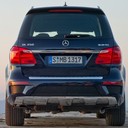
\includegraphics[width=0.14\textwidth]{pictures/pos_1.png}}
\hspace{2mm}
\subfloat{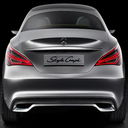
\includegraphics[width=0.14\textwidth]{pictures/pos_2.png}}
\hspace{2mm}
\subfloat{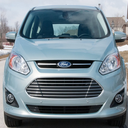
\includegraphics[width=0.14\textwidth]{pictures/pos_3.png}}
\hspace{2mm}
\subfloat{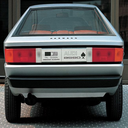
\includegraphics[width=0.14\textwidth]{pictures/pos_4.png}}
\hspace{2mm}
\subfloat{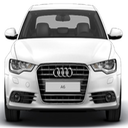
\includegraphics[width=0.14\textwidth]{pictures/pos_5.png}}
\hspace{2mm}
\subfloat{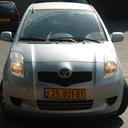
\includegraphics[width=0.14\textwidth]{pictures/pos_6.png}}\\
\subfloat{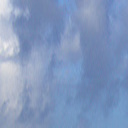
\includegraphics[width=0.14\textwidth]{pictures/neg_1.jpg}}
\hspace{2mm}
\subfloat{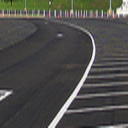
\includegraphics[width=0.14\textwidth]{pictures/neg_2.jpg}}
\hspace{2mm}
\subfloat{
\includegraphics[width=0.14\textwidth]{pictures/neg_3.jpg}}
\hspace{2mm}
\subfloat{
\includegraphics[width=0.14\textwidth]{pictures/neg_4.jpg}}
\hspace{2mm}
\subfloat{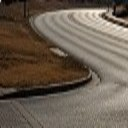
\includegraphics[width=0.14\textwidth]{pictures/neg_5.jpg}}
\hspace{2mm}
\subfloat{
\includegraphics[width=0.14\textwidth]{pictures/neg_6.jpg}}
\caption{Examples of positive and negative training examples for front/rear car detector.}
\label{fig:pos_neg_examples}
\end{figure}

For the reason that the car's view depends on the angle of view, we assemble
positive training data for different angles of the cars. We prepare training
samples for four distinct views of the cars --- front, back and both left and
right sides.

The sides of the car are invariant under the mirror transformation. This
allows to use the same image for training a classifier for each side which
simplifies the training data generation. Front and back of the car, though
different to human point of view, seem to be similar in the HOG visualization.
Therefore, the corresponding datasets can be combined into one.

These datasets contain respectively images of sizes $128 \times 128$ pixels
for front/rear car view and $128 \times 64$ pixels for side view. We utilize
682 positive images that contain cars for training the front/rear detector. In
addition to these positive examples we also convene 7972 negative images. Some
examples from the front/rear positive and negative training datasets are
presented in Figure~\ref{fig:pos_neg_examples}.

The positive examples contain exclusively views of the cars. Each positive
example shows one and only one car. The car occupies the full area of the
image. The photos of the cars depict them centered and seen from the same
angle of view. This is crucial for training a meaningful classifier.

The positive dataset is assembled from different sources: INRIA Car Dataset
by~\citet{inriadata}, Motorway Car Dataset by~\citet{TMEMotorwayDataset}, UIUC
Image Database for Car Detection by~\citet{agarwal2002uiuc}, KITTI car dataset
by~\citet{Geiger2013IJRR} and various car images found in a public domain via
a web searching engine.

In order to create the negative set we randomly sample different sized patches
of the given aspect-ratio ($128 \times 128$ and $128 \times 64$ respectively)
from the images that contain no cars. Following the work of~\citet{dalal2005}
we cut false detections that appear in the first runs of training the
classifier with a clipping tool~\cite{imageclipper} and add them to the
negative training dataset.

We use the trained classifier on the images from the camera mounted inside of
the car facing sidewards or, possibly, onto any other moving platform. During
our experiments we use a Bumblebee stereo-camera
(Figure~\ref{subfig:bumblebee}) pointed to the side of the Europa robot Obelix
(Figure~\ref{subfig:obelix}).

\begin{figure}[t]%
\centering
\subfloat{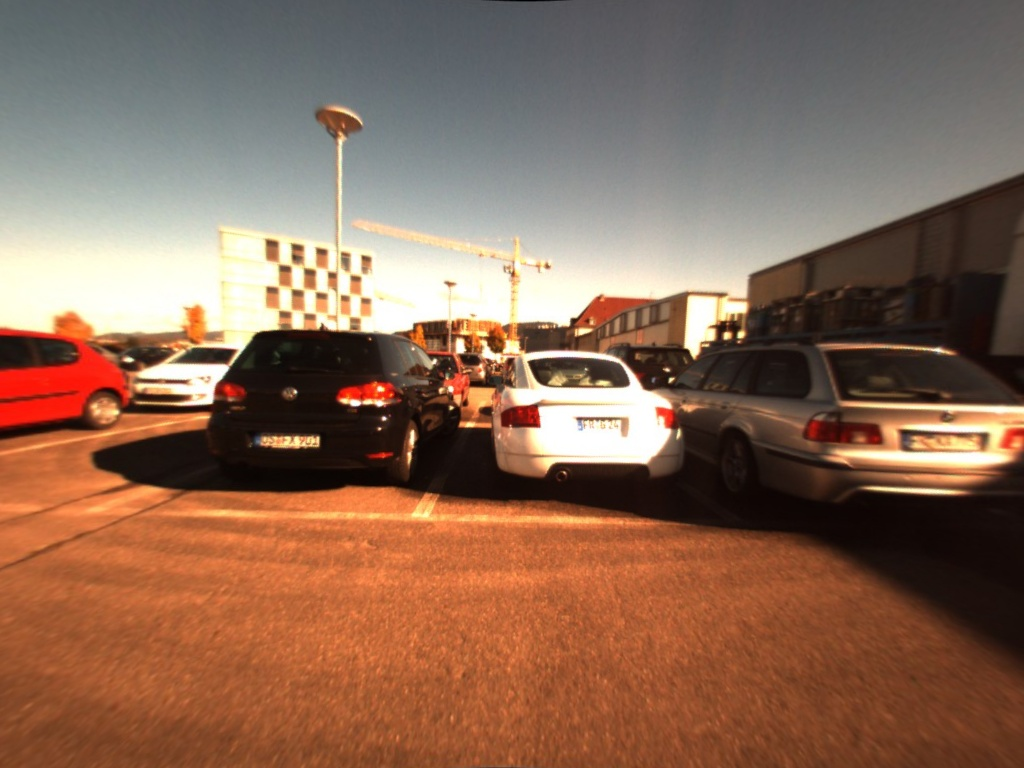
\includegraphics[width=0.31\textwidth]{pictures/left.jpg}}\hspace{2mm}
\subfloat{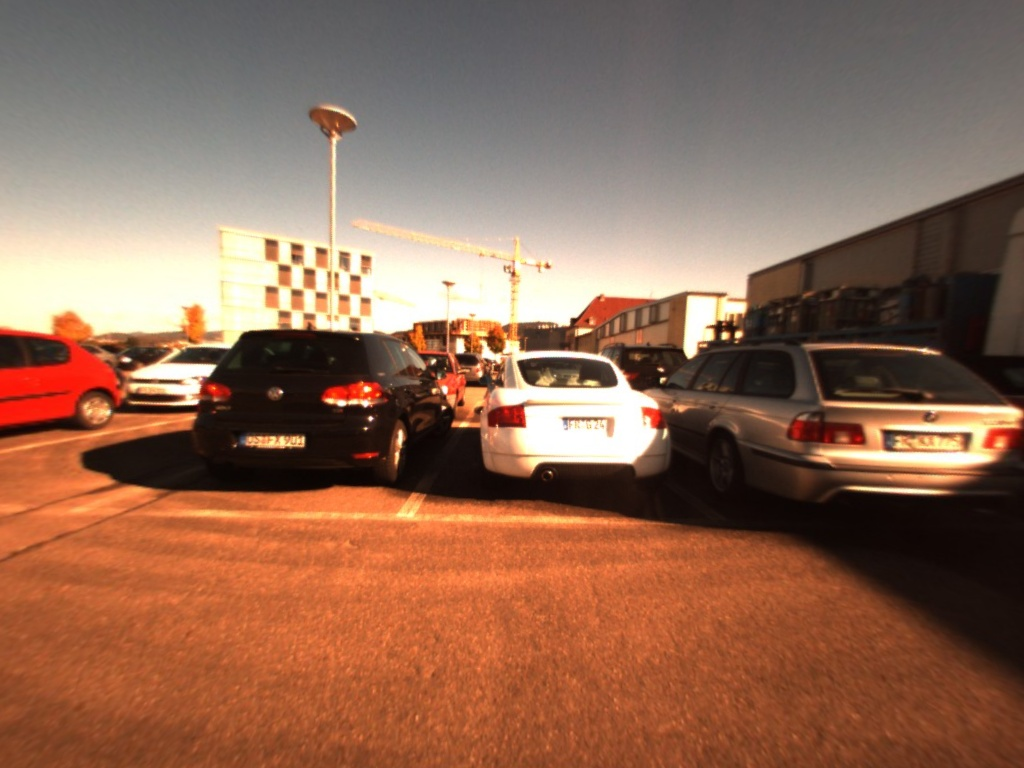
\includegraphics[width=0.31\textwidth]{pictures/right.jpg}}\hspace{2mm}
\subfloat{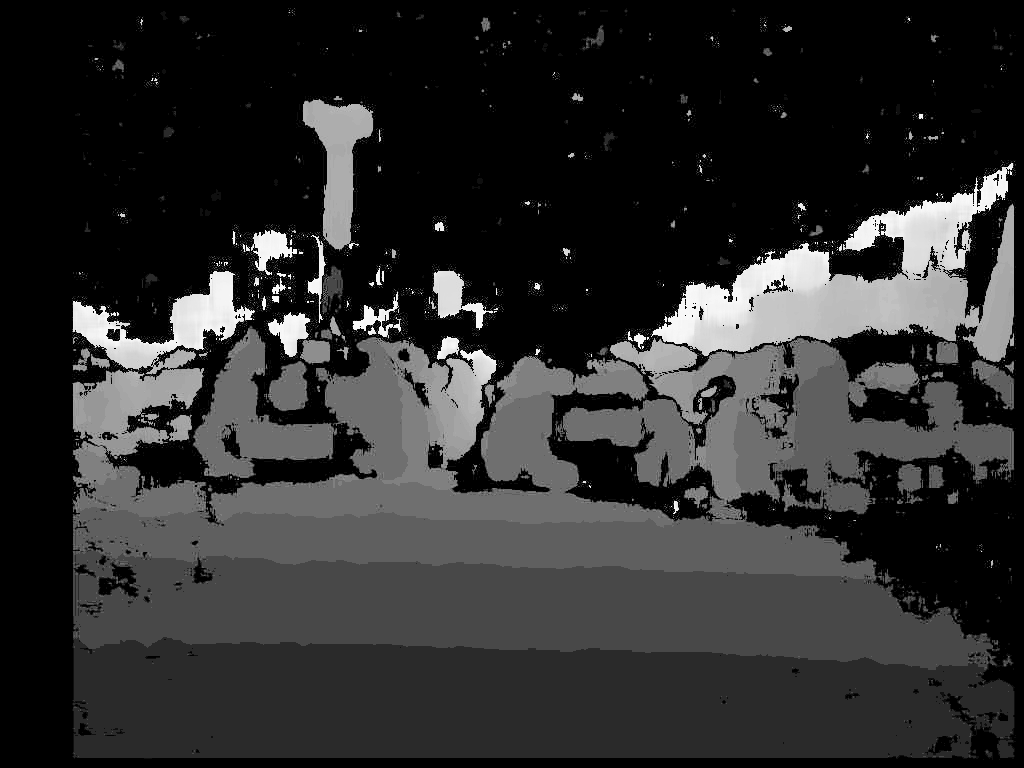
\includegraphics[width=0.31\textwidth]{pictures/depth.png}}\\
\caption{Depth acquired from disparity between stereo images.}
\label{fig:depth_from_disparity}
\end{figure}

We are interested in detections accumulated over time. The same car is seen
from different angles, throughout different (usually consequent) images. We
consider the car to be detected if it has been detected at least once in the
sequence of images, featuring this particular car. With this in mind, the
detection rate for our realization of the approach is approximately 95\%.

The examples of detected cars can be seen in
Figure~\ref{fig:detection_examples}.

\begin{figure}[t]
\centering
\begin{tabular}{cc}
\subfloat[]{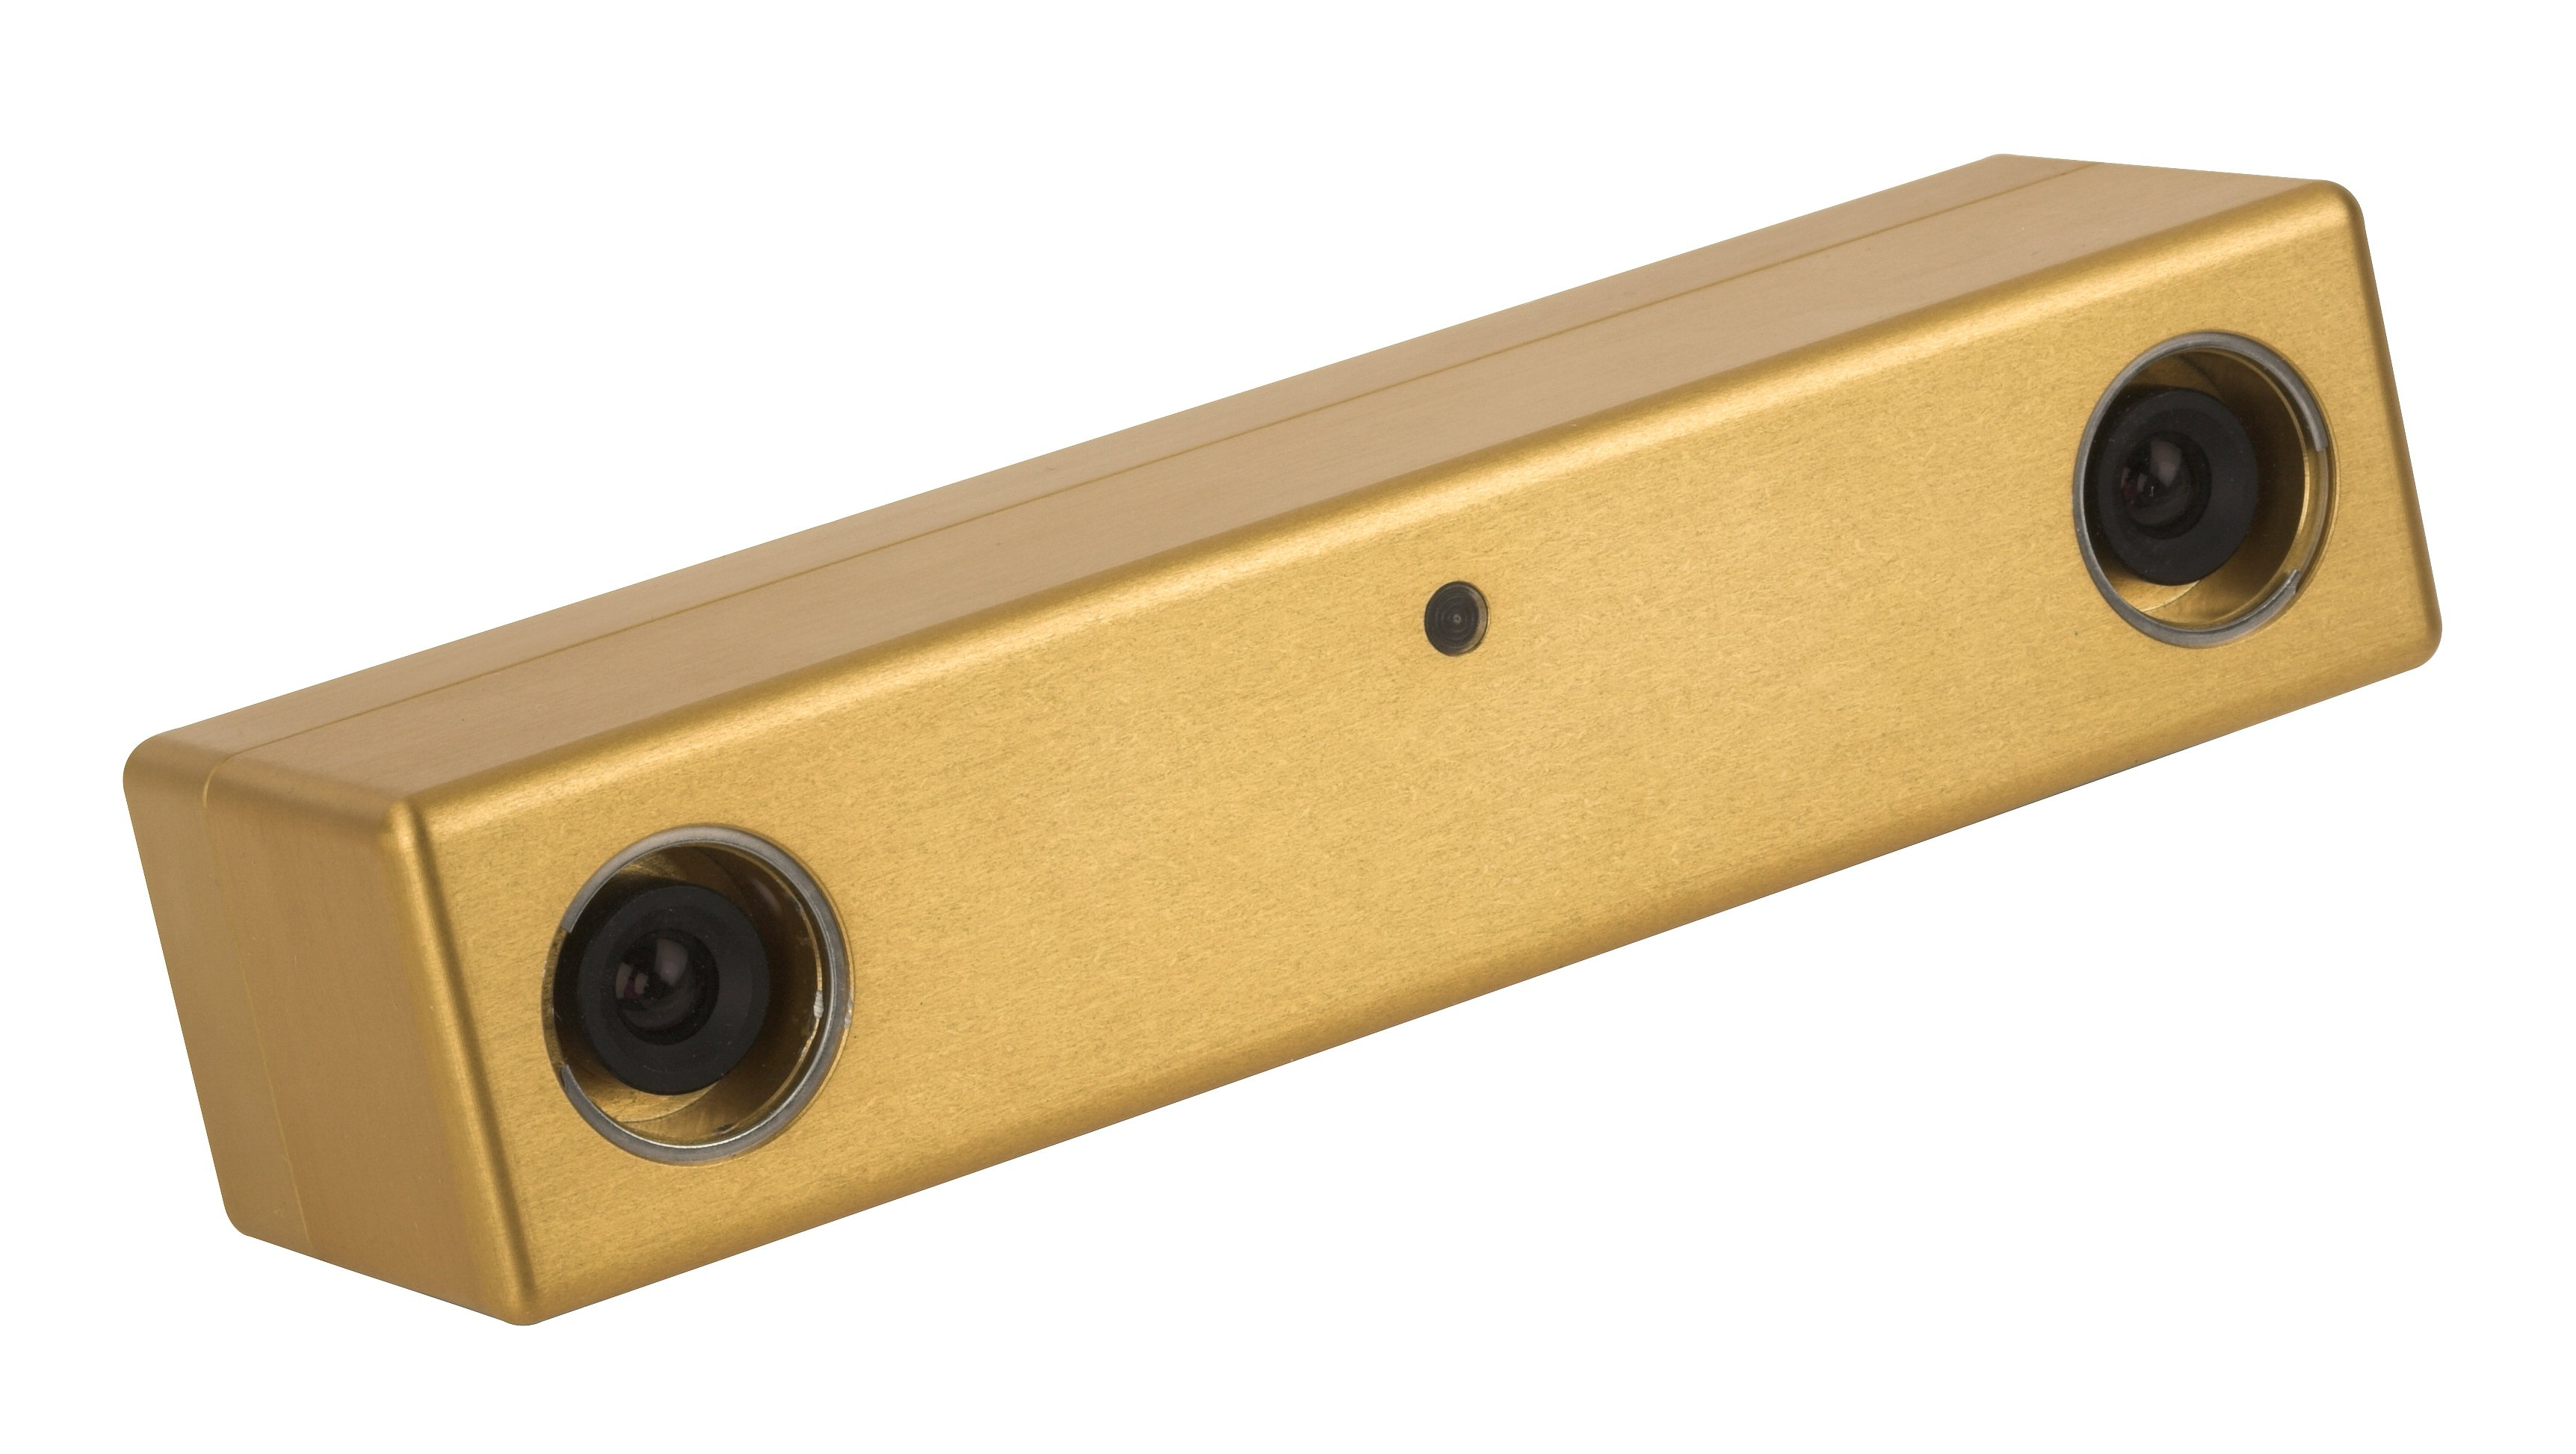
\includegraphics[width=3cm]{pictures/bumblebee.jpg}\label{subfig:bumblebee}}\vspace{4mm} \\
\subfloat[]{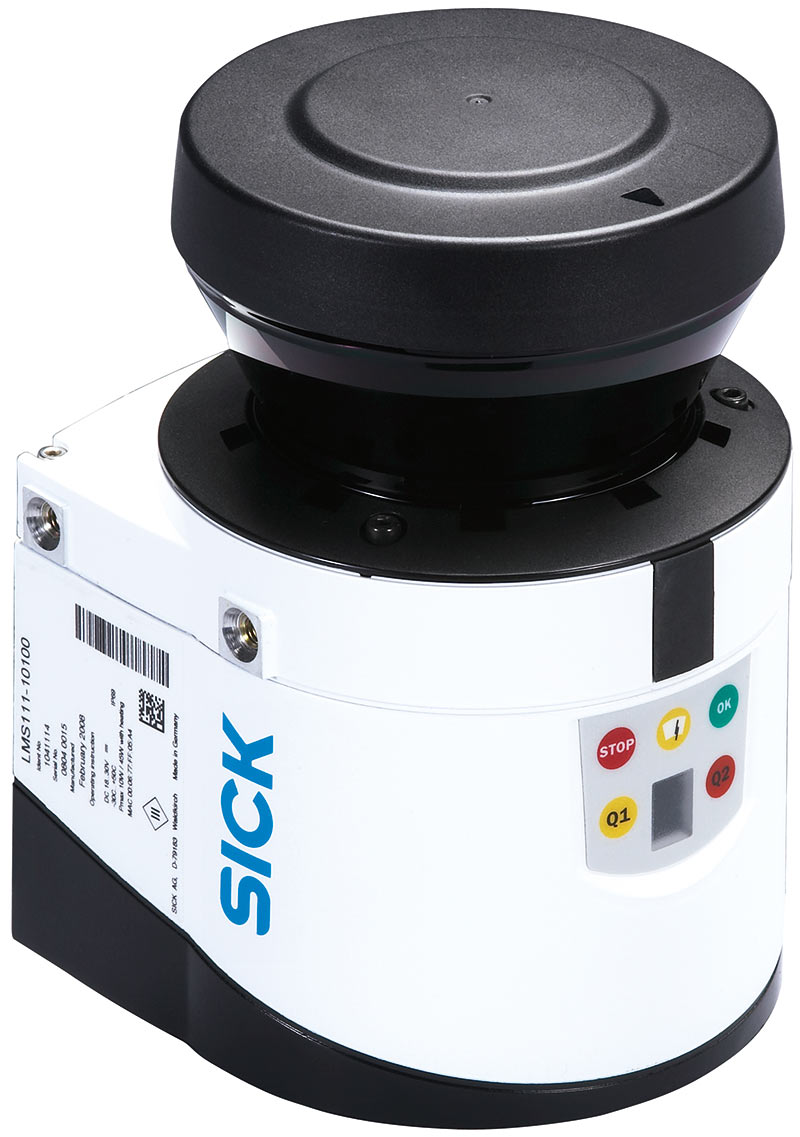
\includegraphics[width=2cm]{pictures/lms_2_0.jpg}\label{subfig:laser}} &
\multirow{-12}[3]{*}{\subfloat[]{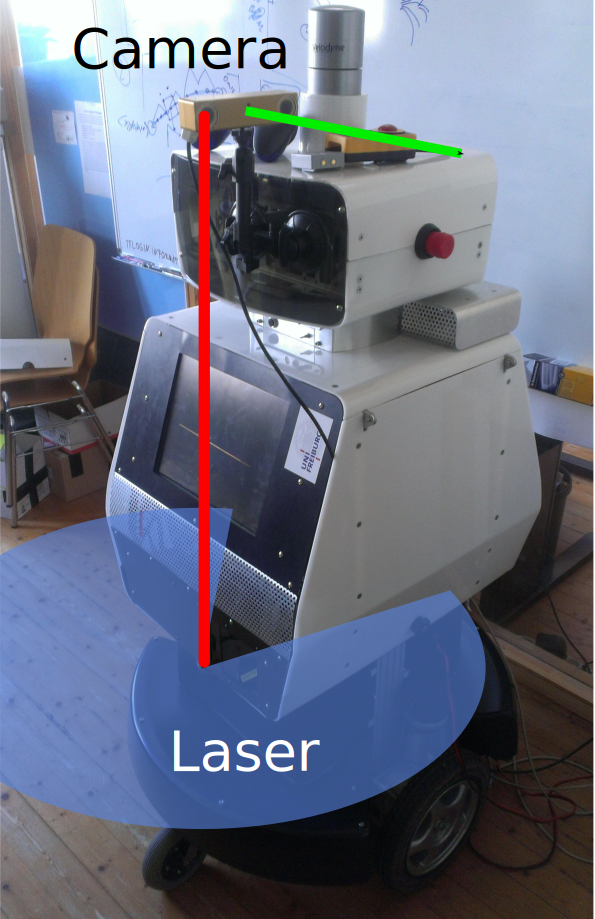
\includegraphics[width=4cm]{pictures/obelix.pdf}\label{subfig:obelix}}} \\
\end{tabular}
\caption{A Bumblebee stereo camera \subref{subfig:bumblebee} and a laser range finder \subref{subfig:laser} mounted on the Obelix robot on the same vertical axis \subref{subfig:obelix}.}
\end{figure}


\begin{figure}[p]%
\centering
\subfloat{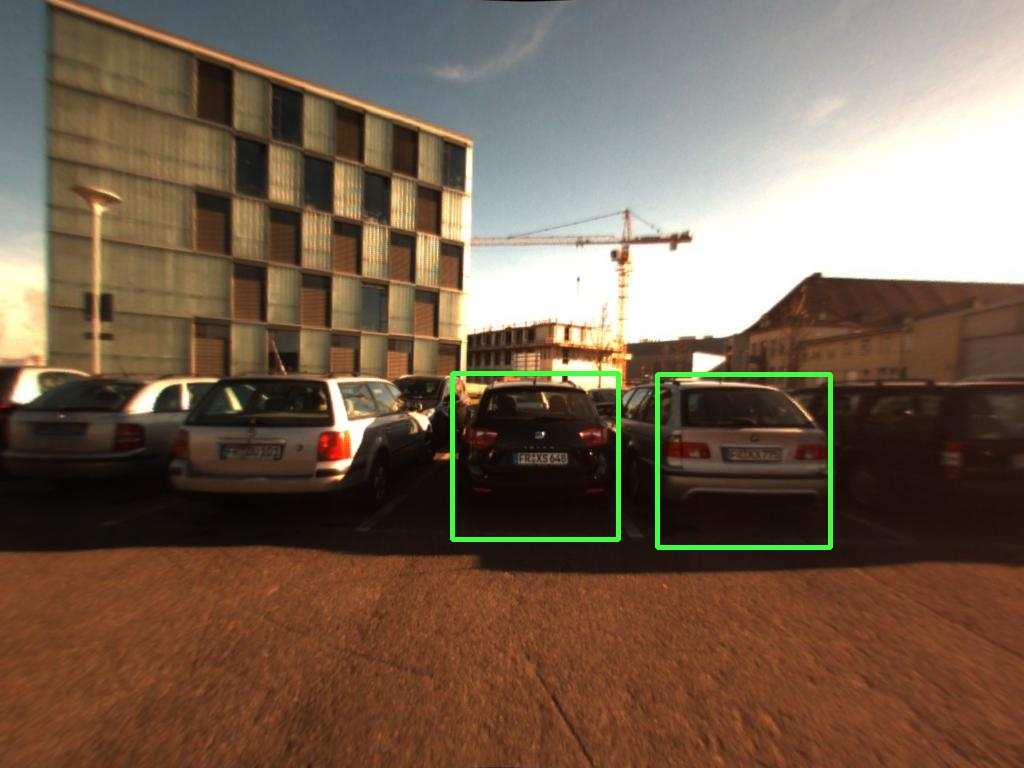
\includegraphics[width=0.3\textwidth]{pictures/det_1.jpg}}\hspace{2mm}
\subfloat{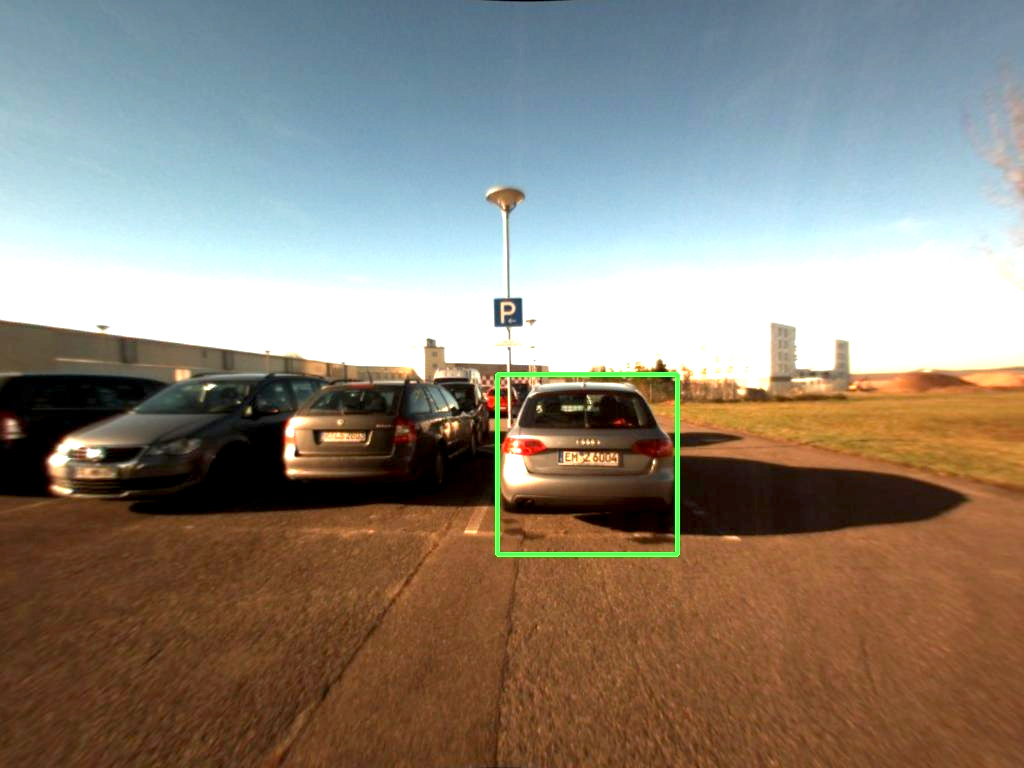
\includegraphics[width=0.3\textwidth]{pictures/det_2.jpg}}\hspace{2mm}
\subfloat{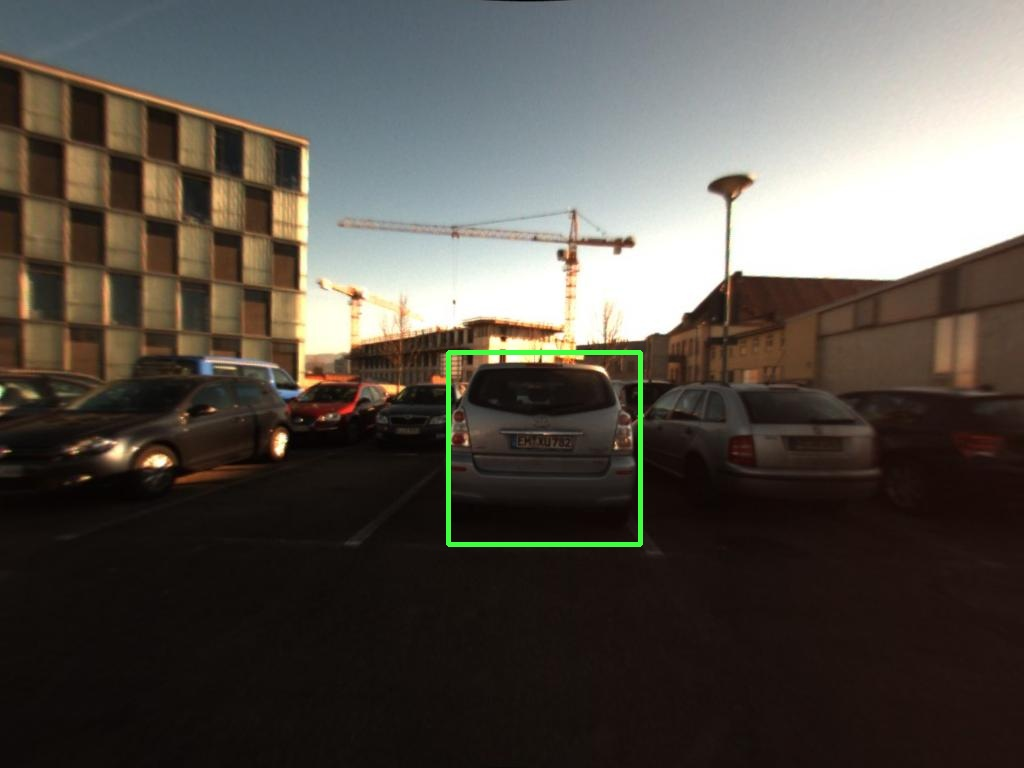
\includegraphics[width=0.3\textwidth]{pictures/det_3.jpg}}\\
\subfloat{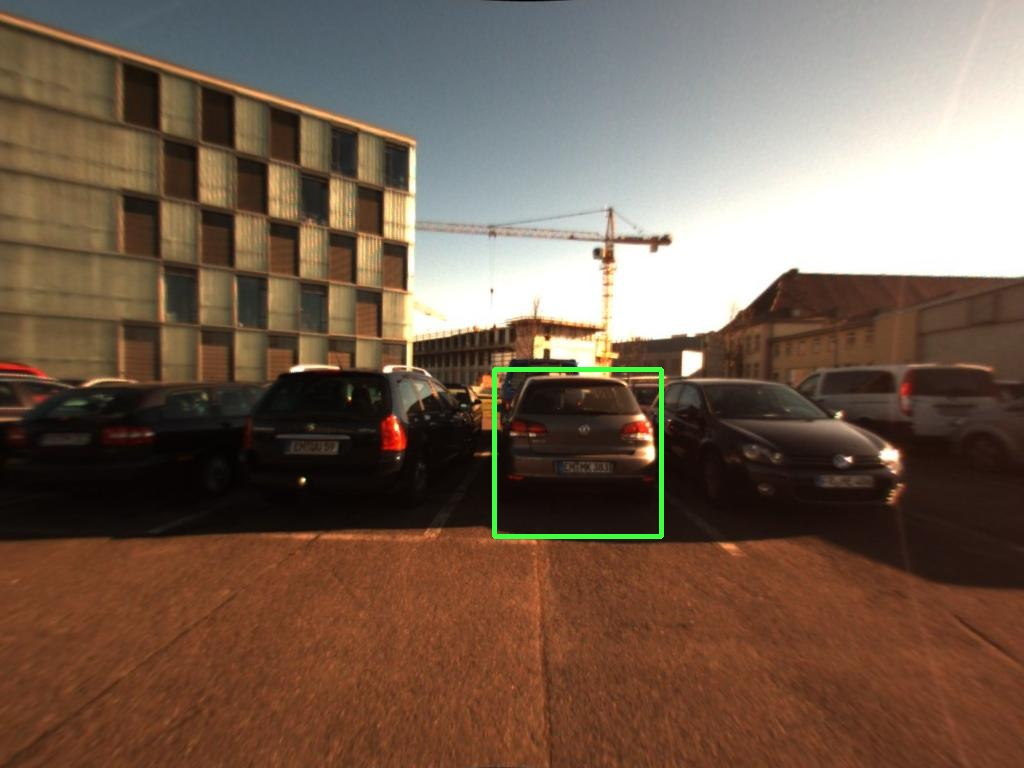
\includegraphics[width=0.3\textwidth]{pictures/det_4.jpg}}\hspace{2mm}
\subfloat{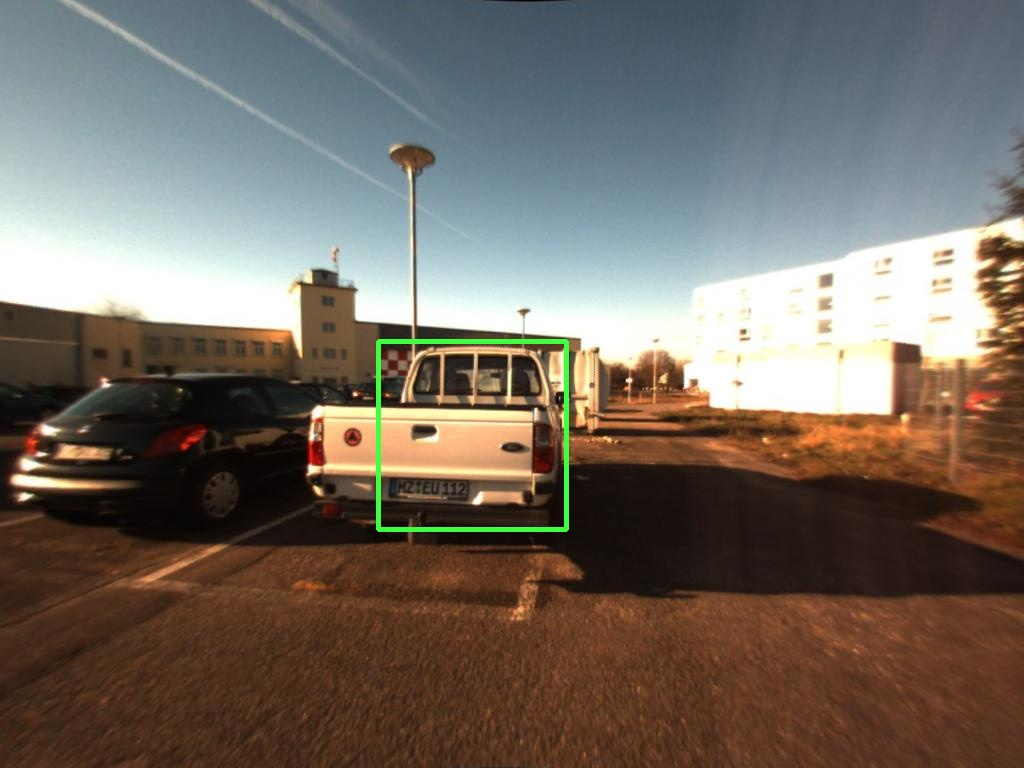
\includegraphics[width=0.3\textwidth]{pictures/det_5.jpg}}\hspace{2mm}
\subfloat{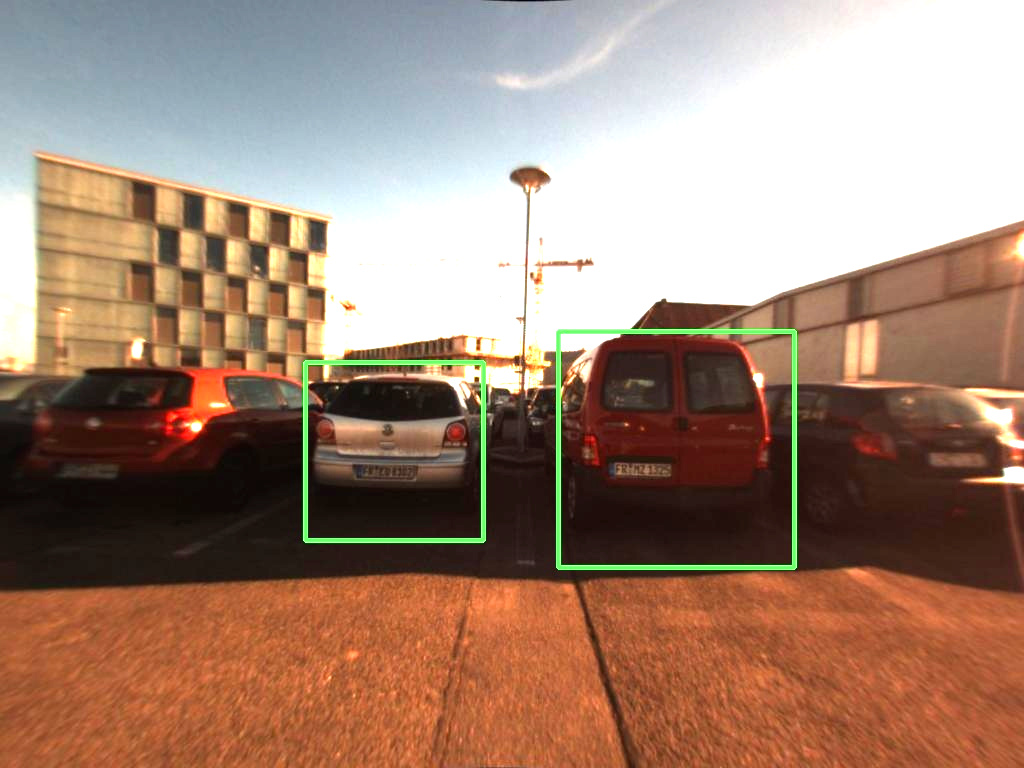
\includegraphics[width=0.3\textwidth]{pictures/det_6.jpg}}\\
\subfloat{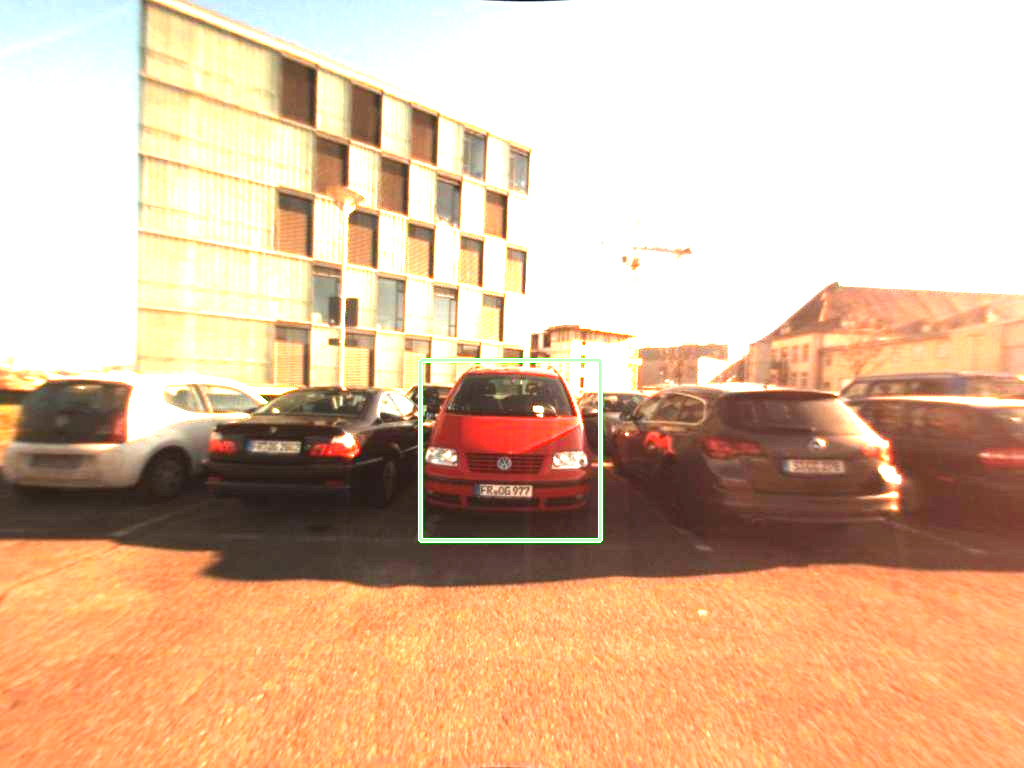
\includegraphics[width=0.3\textwidth]{pictures/det_7.jpg}}\hspace{2mm}
\subfloat{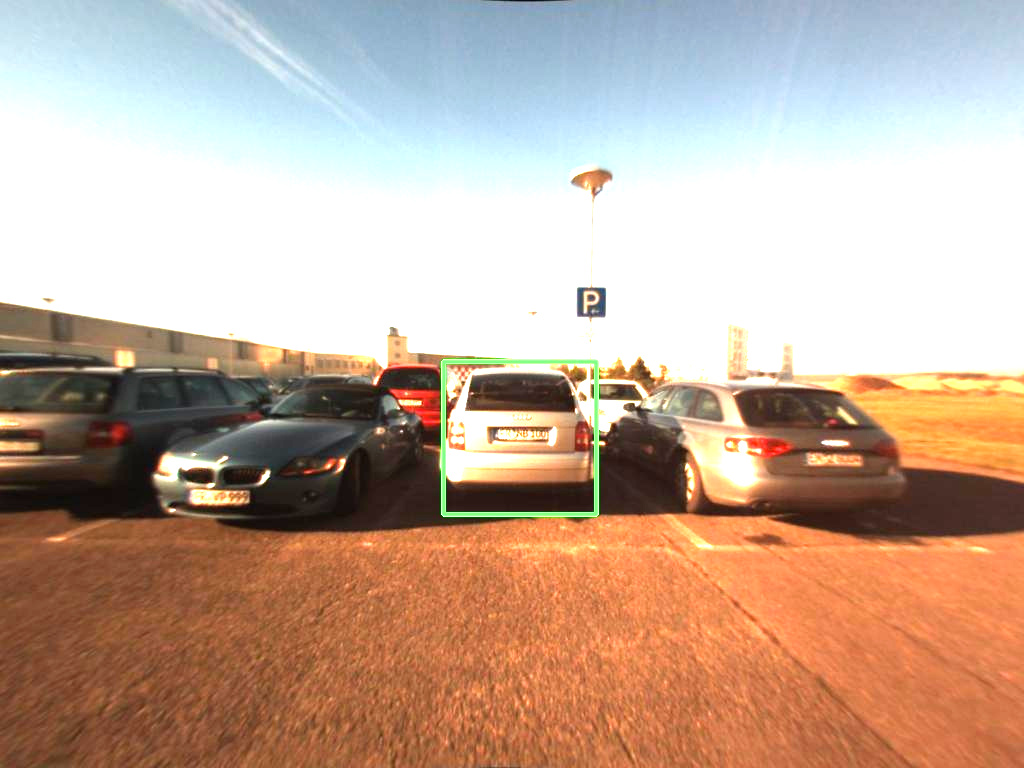
\includegraphics[width=0.3\textwidth]{pictures/det_8.jpg}}\hspace{2mm}
\subfloat{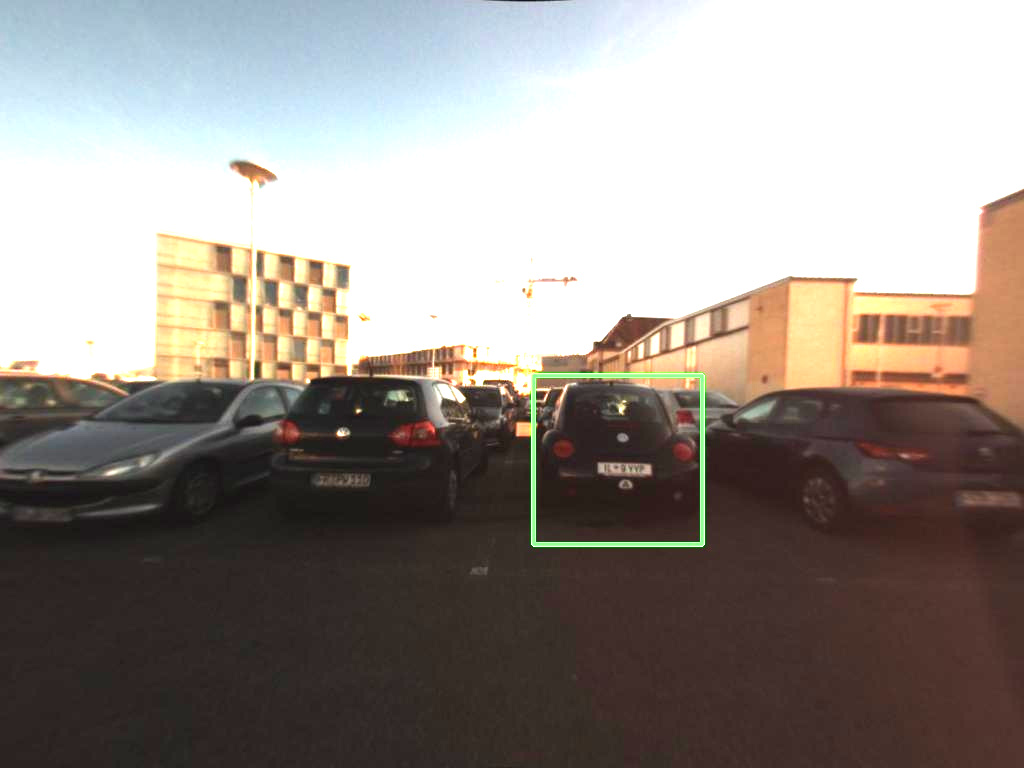
\includegraphics[width=0.3\textwidth]{pictures/det_9.jpg}}\\
\subfloat{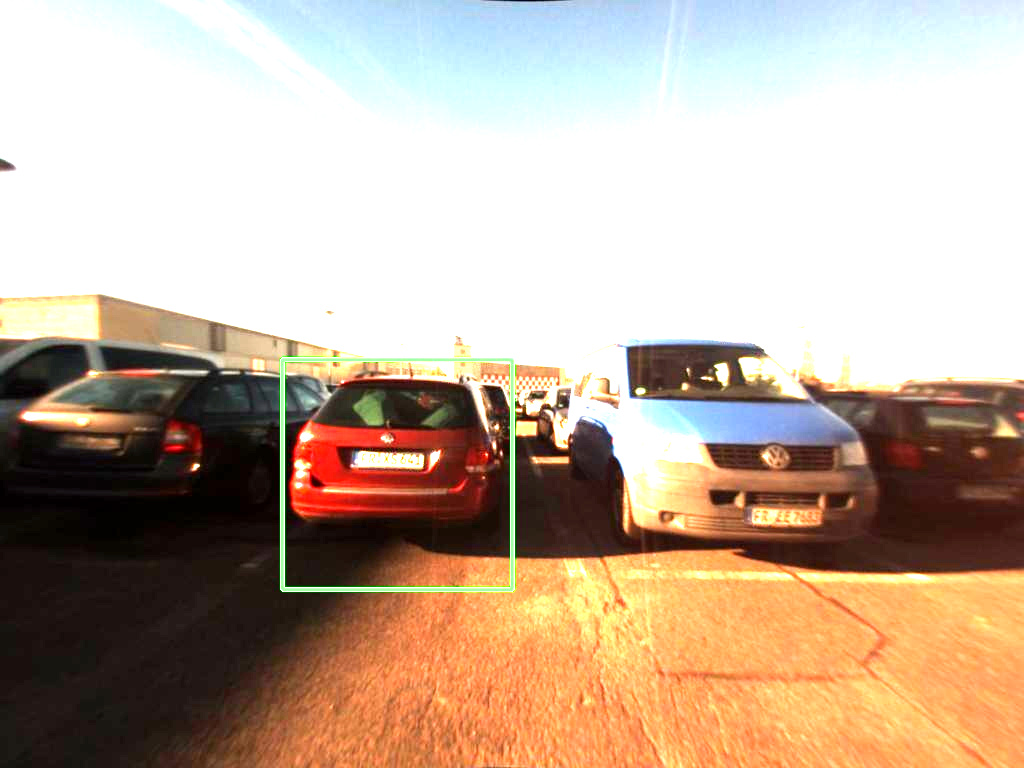
\includegraphics[width=0.3\textwidth]{pictures/det_10.jpg}}\hspace{2mm}
\subfloat{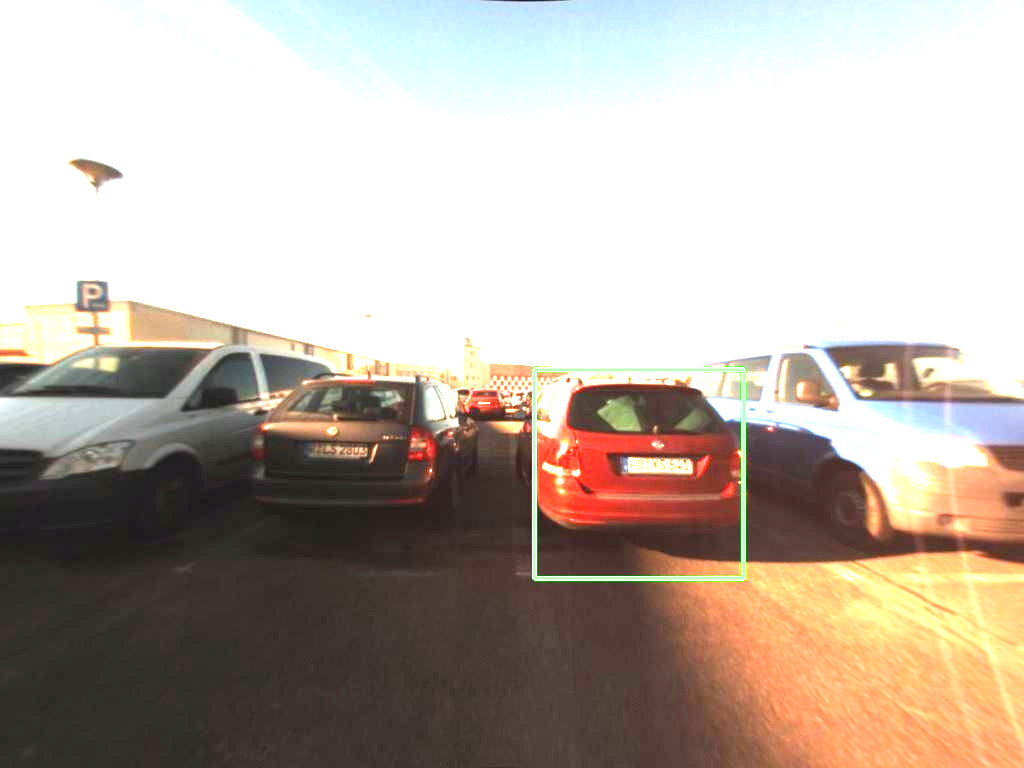
\includegraphics[width=0.3\textwidth]{pictures/det_11.jpg}}\hspace{2mm}
\subfloat{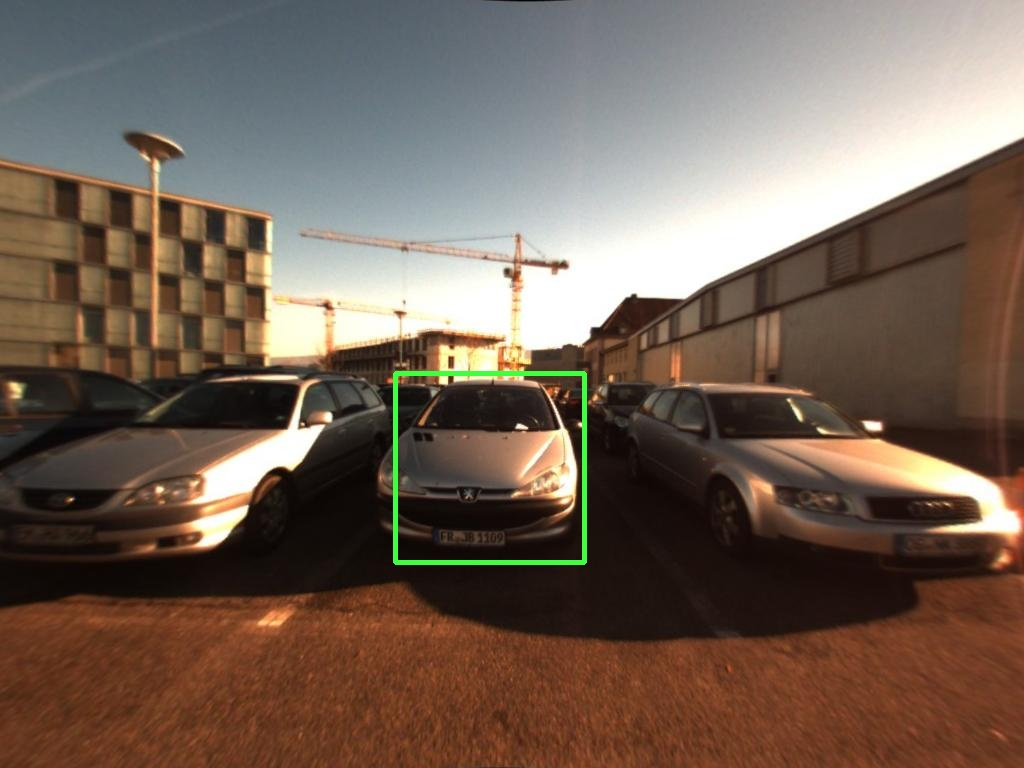
\includegraphics[width=0.3\textwidth]{pictures/det_12.jpg}}\\
\subfloat{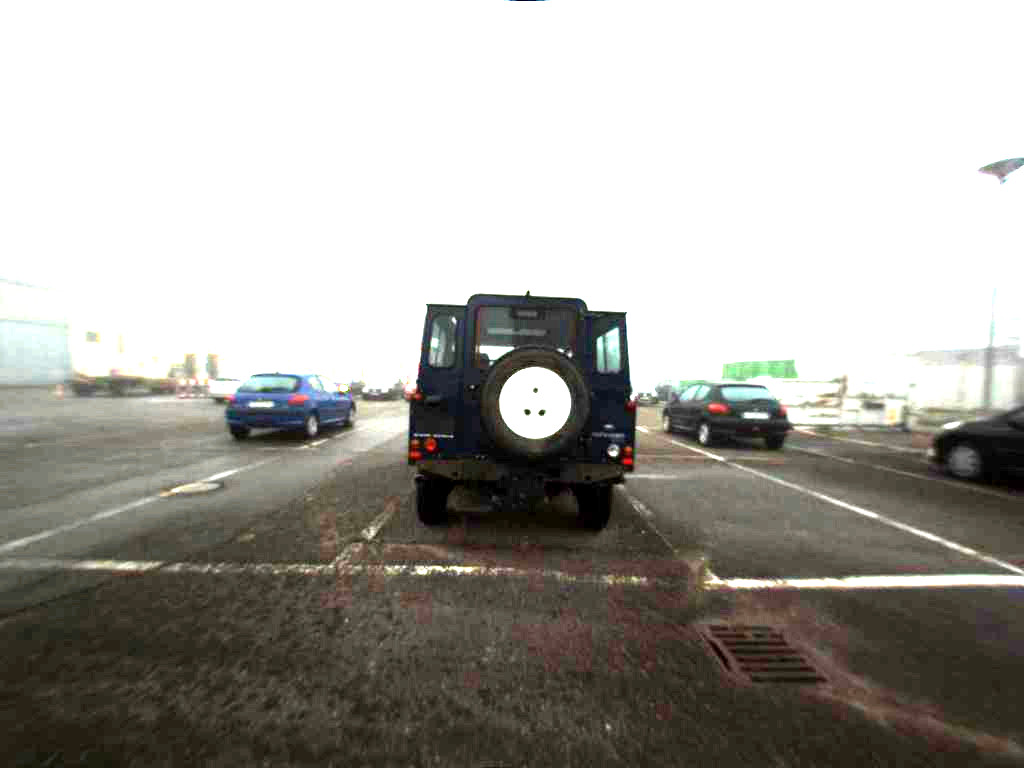
\includegraphics[width=0.3\textwidth]{pictures/undet_1.jpg}}\hspace{2mm}
\subfloat{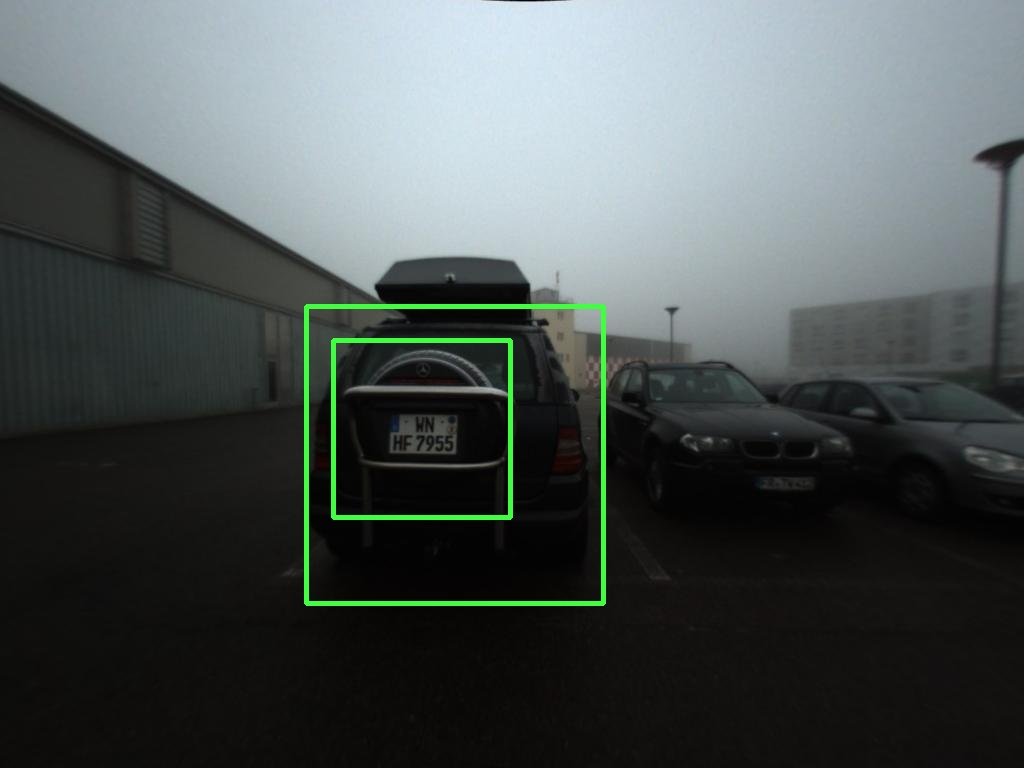
\includegraphics[width=0.3\textwidth]{pictures/undet_2.jpg}}\hspace{2mm}
\subfloat{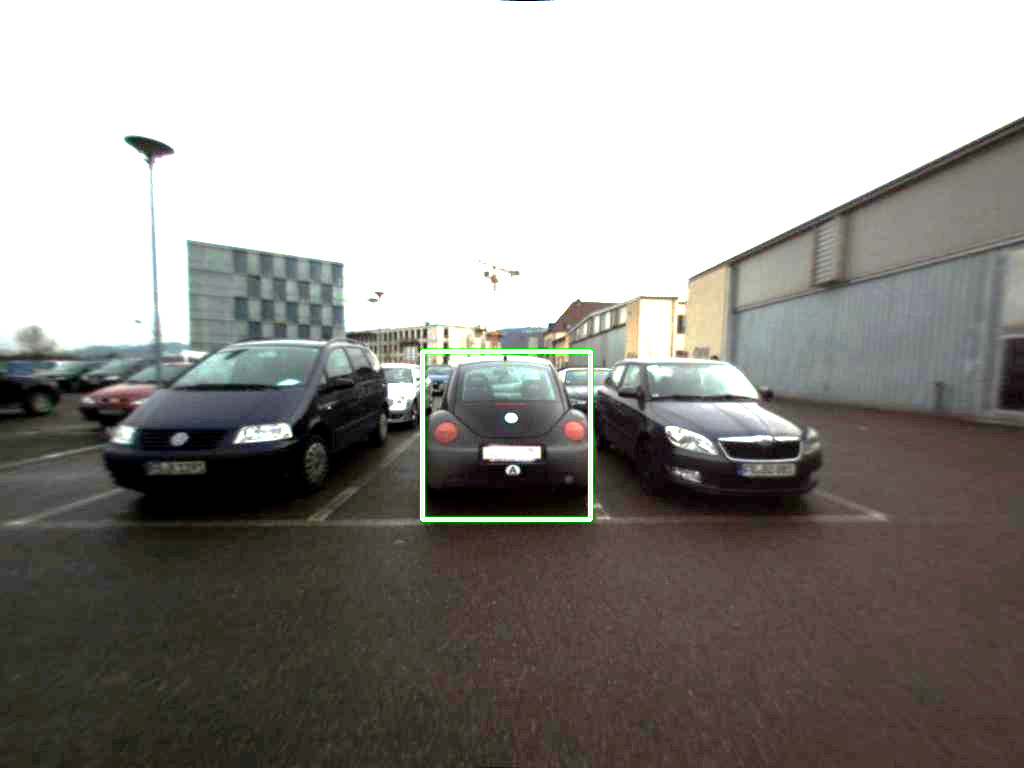
\includegraphics[width=0.3\textwidth]{pictures/det_14.jpg}}\\
\caption{Examples of detections of different cars under different light conditions.}
\label{fig:detection_examples}
\end{figure}

% section visual_car_detection (end)

\section{Parking Lot Modeling}
\label{sec:parking_lots_modeling}

\begin{figure}[p]%
\centering
\subfloat[Aerial view.]{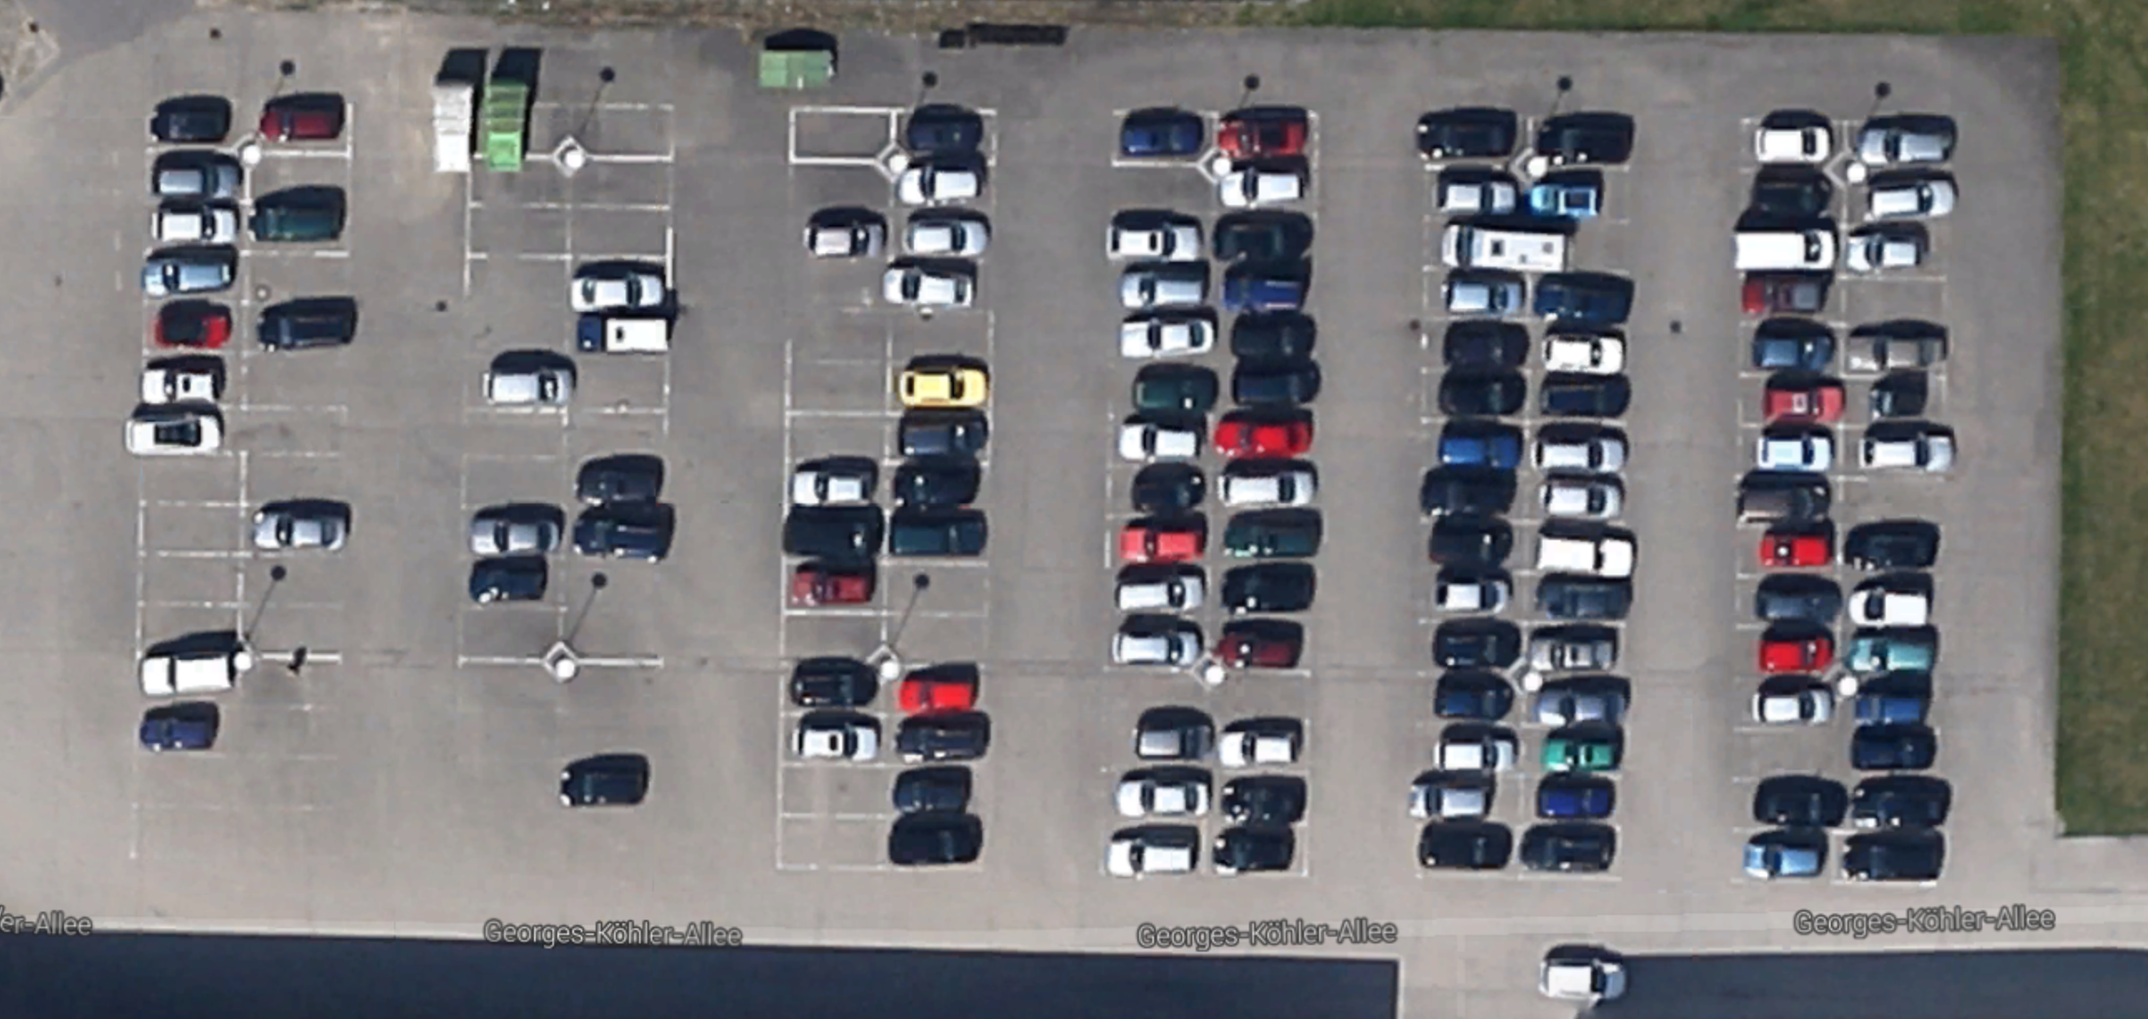
\includegraphics[width=0.6\textwidth]{pictures/google_map.pdf}\label{subfig:aerial}} \\
\subfloat[Car detections over the map built with the laser-based SLAM procedure.]{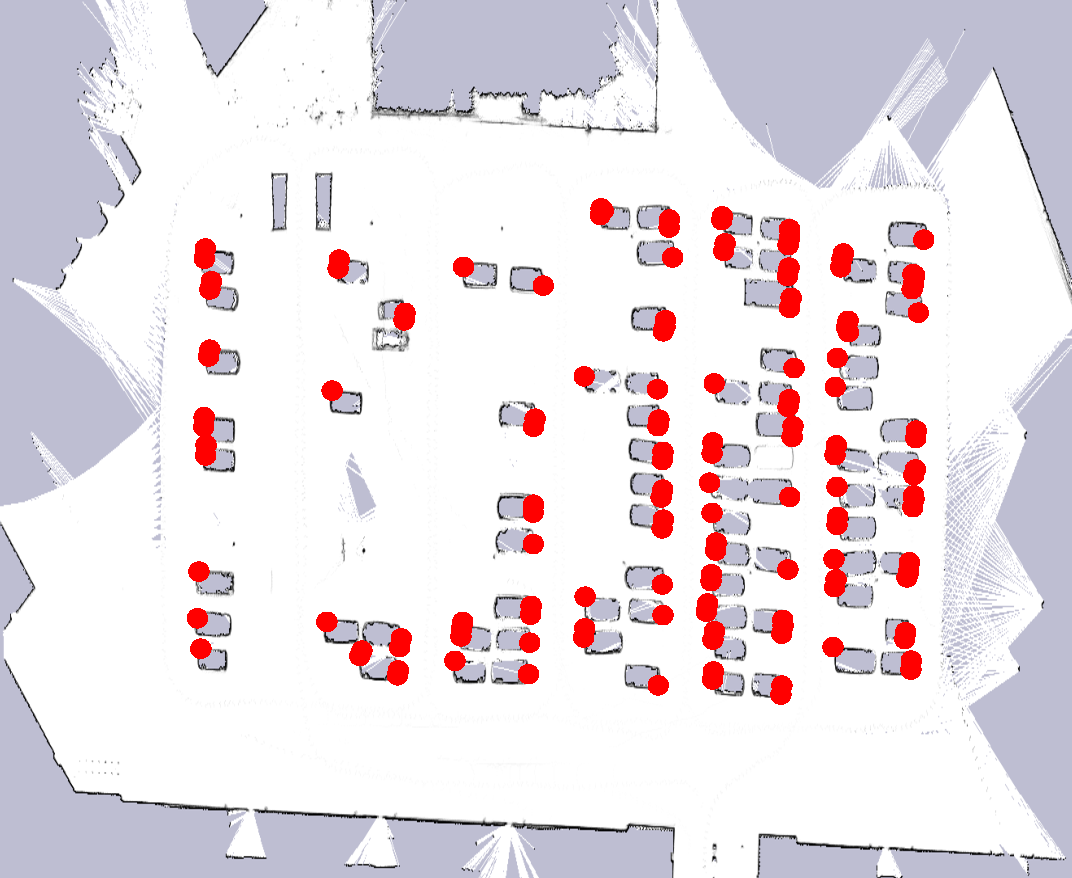
\includegraphics[width=0.6\textwidth]{pictures/laser_fusion.pdf}\label{subfig:slam_detections}} \\
\subfloat[Occupancy grid map acquired as described in Section~\ref{sub:occupancy_grids}.]{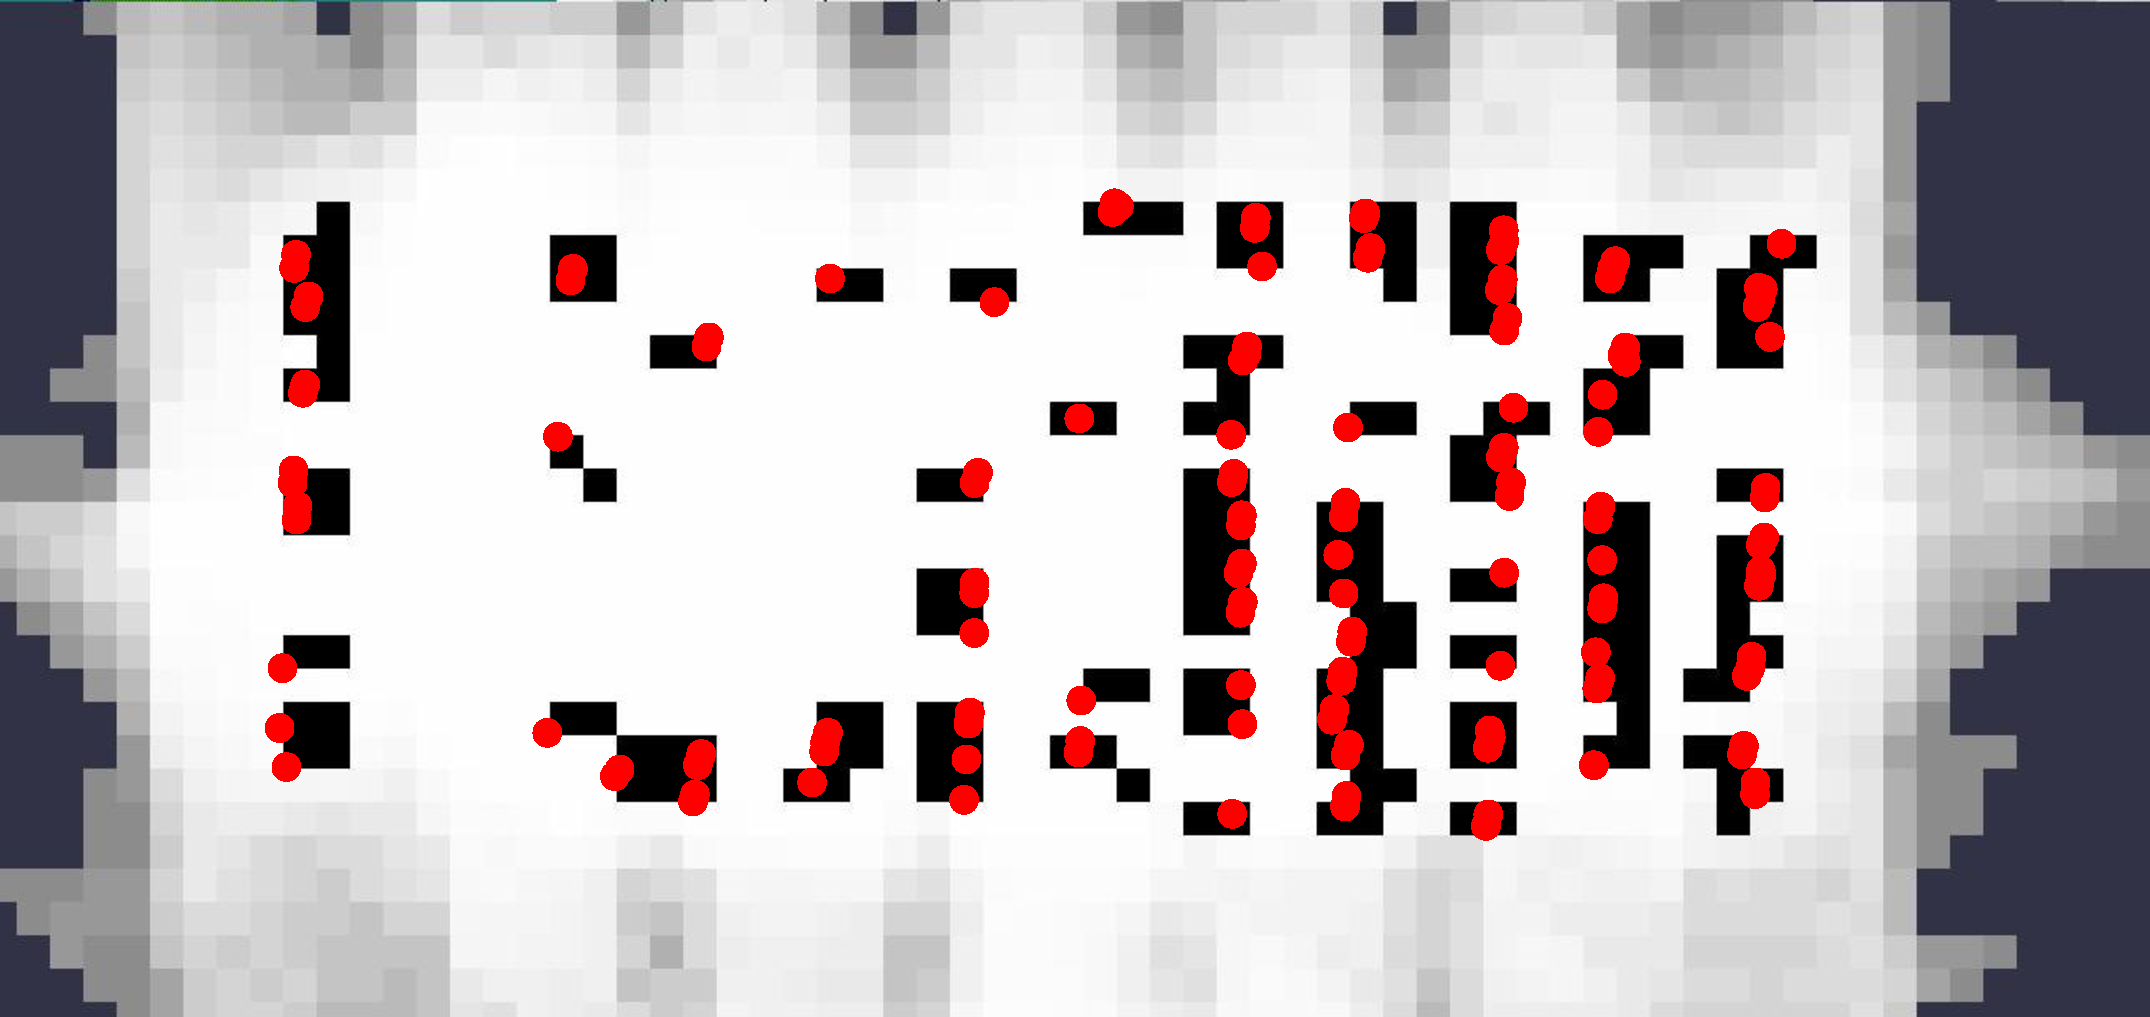
\includegraphics[width=0.6\textwidth]{pictures/occupancy_cars.pdf}\label{subfig:occ_maps_detections}} \\
\subfloat[Cars positions mapped to pre-defined parking lot positions.]{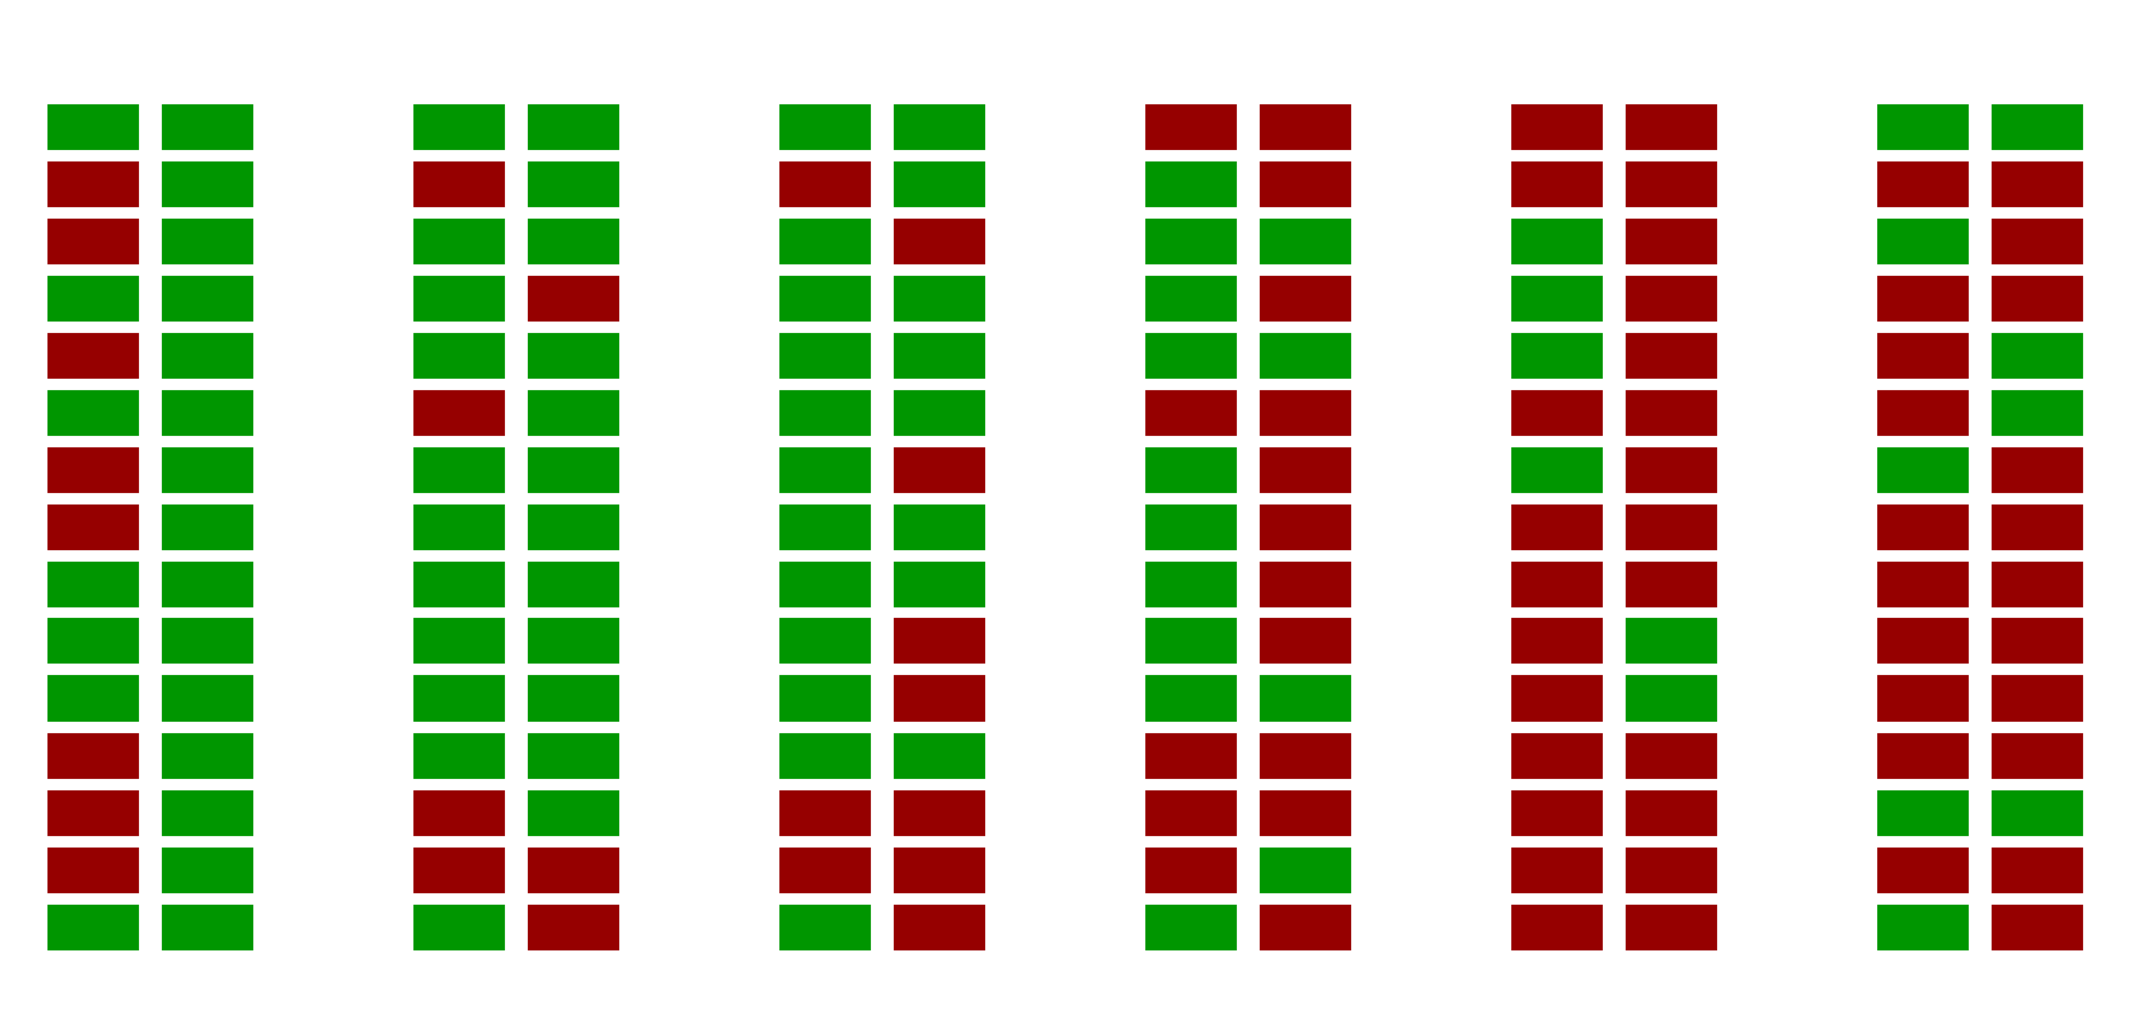
\includegraphics[width=0.6\textwidth]{pictures/parking_lots_detections.pdf}\label{subfig:pre_defined}}
\caption{Representations of the campus parking lot at the university of Freiburg. \\ Images \subref{subfig:slam_detections}, \subref{subfig:occ_maps_detections},~\subref{subfig:pre_defined}  represent the same occupancy state of the parking lot.}
\label{fig:different_mappings}
\end{figure}

The occupancy data is based on the 2D data obtained either from the stereo
cameras (Figure~\ref{subfig:bumblebee}) or from laser range finder, mounted on
the robot (Figure~\ref{subfig:laser}). As can be seen in the figure, the
stereo camera is mounted on the same z-axis with the laser range finder. We
search for the endpoints that represent the cars as described in the section
\nameref{sec:perception} of chapter \nameref{cha:our_approach}.

Figure~\ref{fig:depth_from_disparity} shows that the depth information
computed from the disparity image between two stereo images lacks precision
and has a significant amount of noise. Not only this noise is caused by the
method of depth estimation and errors in point association, but it also
suffers from the windows present in almost any car. The windows are
transparent which results in wrong depth measurements present in the detected
regions of interest.

To avoid the high noise from the stereo camera, we use the depth measurements
from a laser range finder. Each laser measurement has high precision in
measuring the distance. Because of its mounting position on the human knee
level, it also does not suffer from the partial transparency of the cars as
individual laser beams never encounter the cars' windows.

We present occupancy data aggregated to the occupancy grids as well as into
pre-defined parking lot positions. The illustration of differences in the maps
representations can be seen in Figure~\ref{fig:different_mappings}. The figure
shows car detected  cars positions as red dots. We produce these detections
fusing the laser range finder measurements with the visual detections as
described in Chapter~\ref{ssub:laser_range_finder}.

There are two distinct ways in which we model the parking lots: occupancy grid
maps and pre-defined parking lots positions.

As can be seen from the Figure~\ref{subfig:occ_maps_detections} the occupancy
grid based representation lacks precision. The main problem are the
discretization errors. It is a common situation when the detections on
different sides of the same car fall into different grid cells, causing
erroneous map representation. Another problem of the occupancy grid based
approach is an imperfect approximation of the car orientation. We argue, that
using the observation model, as seen in Figure~\ref{fig:maptest}, yields the
orientation of the detected car to be influenced by the angle from which it is
observed.

\begin{figure}[t]
    \begin{center}
        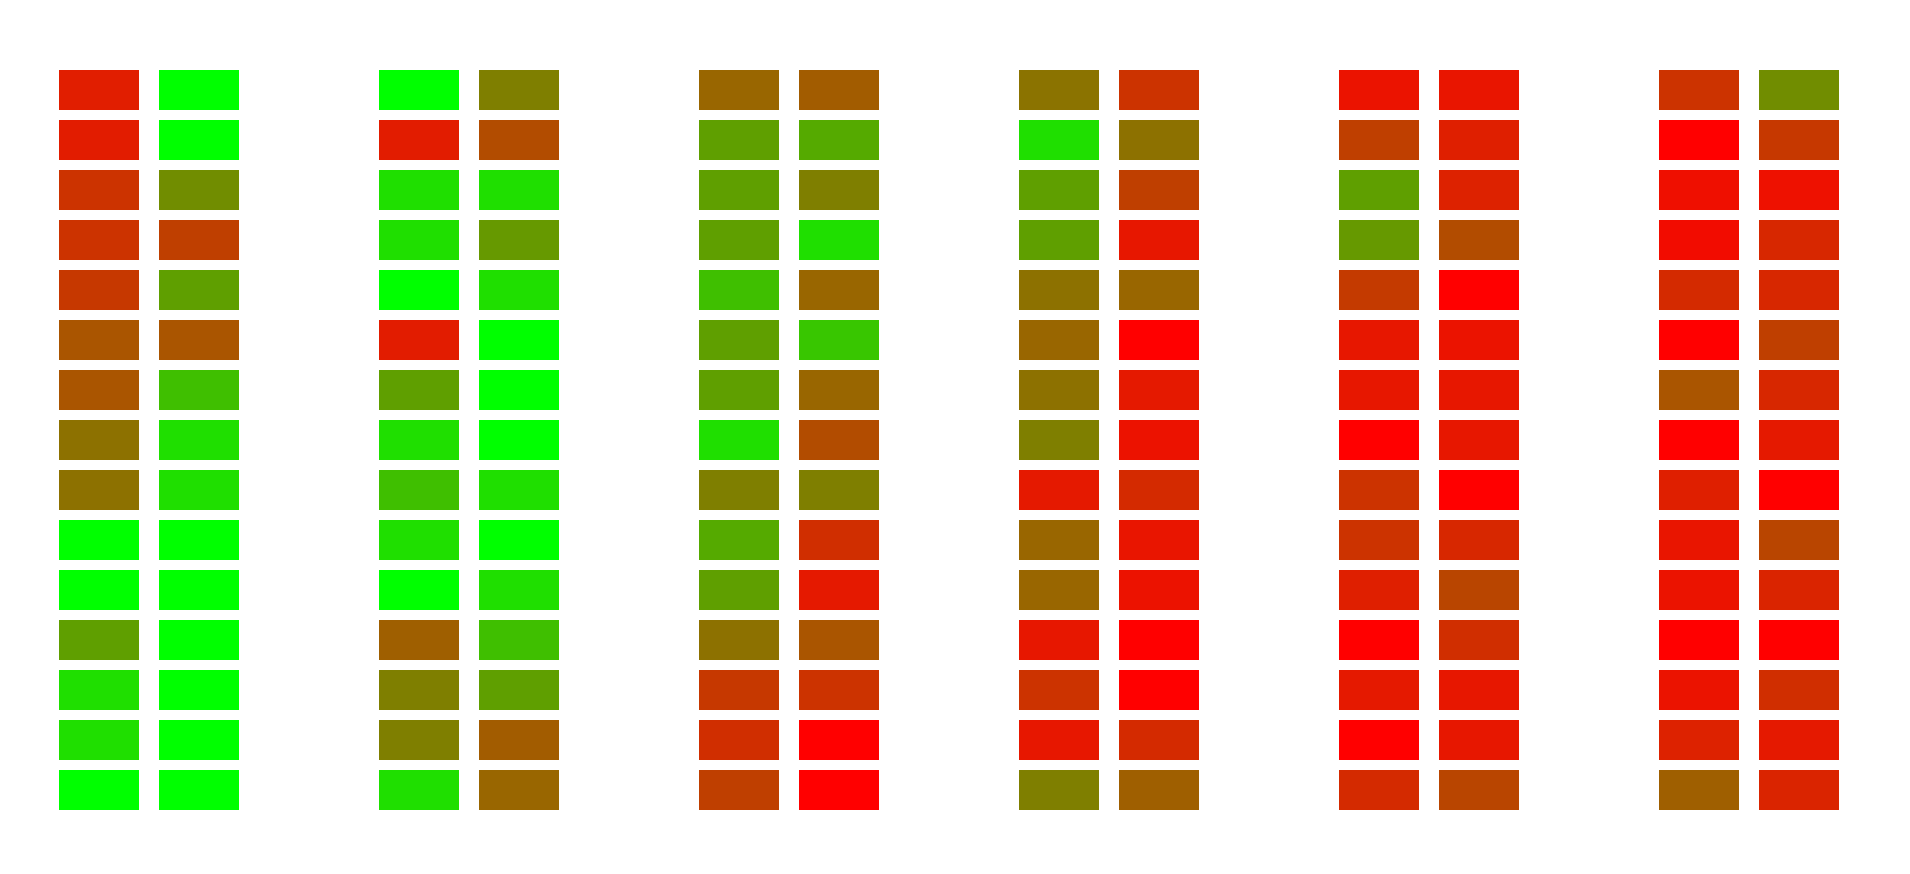
\includegraphics[width=0.6\textwidth]{pictures/parking_lots.png}
    \end{center}
    \caption{Occupancy probability accumulated during a sequence of observations shown in color. The greener the parking lot is --- the bigger the probability for it to be free.}
    \label{fig:occupancy_accumulated}
\end{figure}

Because of these issues, we mostly utilize the pre-defined positions of the
parking lots for occupancy estimation. An example of the occupancy information
from the data gathered during one run is presented in
Figure~\ref{subfig:pre_defined}. The exact positions of the parking lots and
deterministic association of detections to them allows us to quantify the
mapping precision. For this system we measure the detection rate as a relation
of the number of correctly labeled parking lots to the total number of parking
lots. This results in: $\frac{\mathrm{correct}}{\mathrm{correct} +
\mathrm{wrong}} \approx 92\% $ of all parking lots to be labeled correctly as
occupied or free respectively. The biggest source of error is failing to
detect the cars or assigning them to the wrong parking lot. The first problem
comes from the visual visual detection part, that, of course, propagates the
error. The second one is usually due to abnormal sizes of the cars or improper
position in the parking lot.

% section parking_lots_modeling (end)


\section{Action Planning}
\label{sec:planning_results}

\begin{figure}[t]
\begin{center}
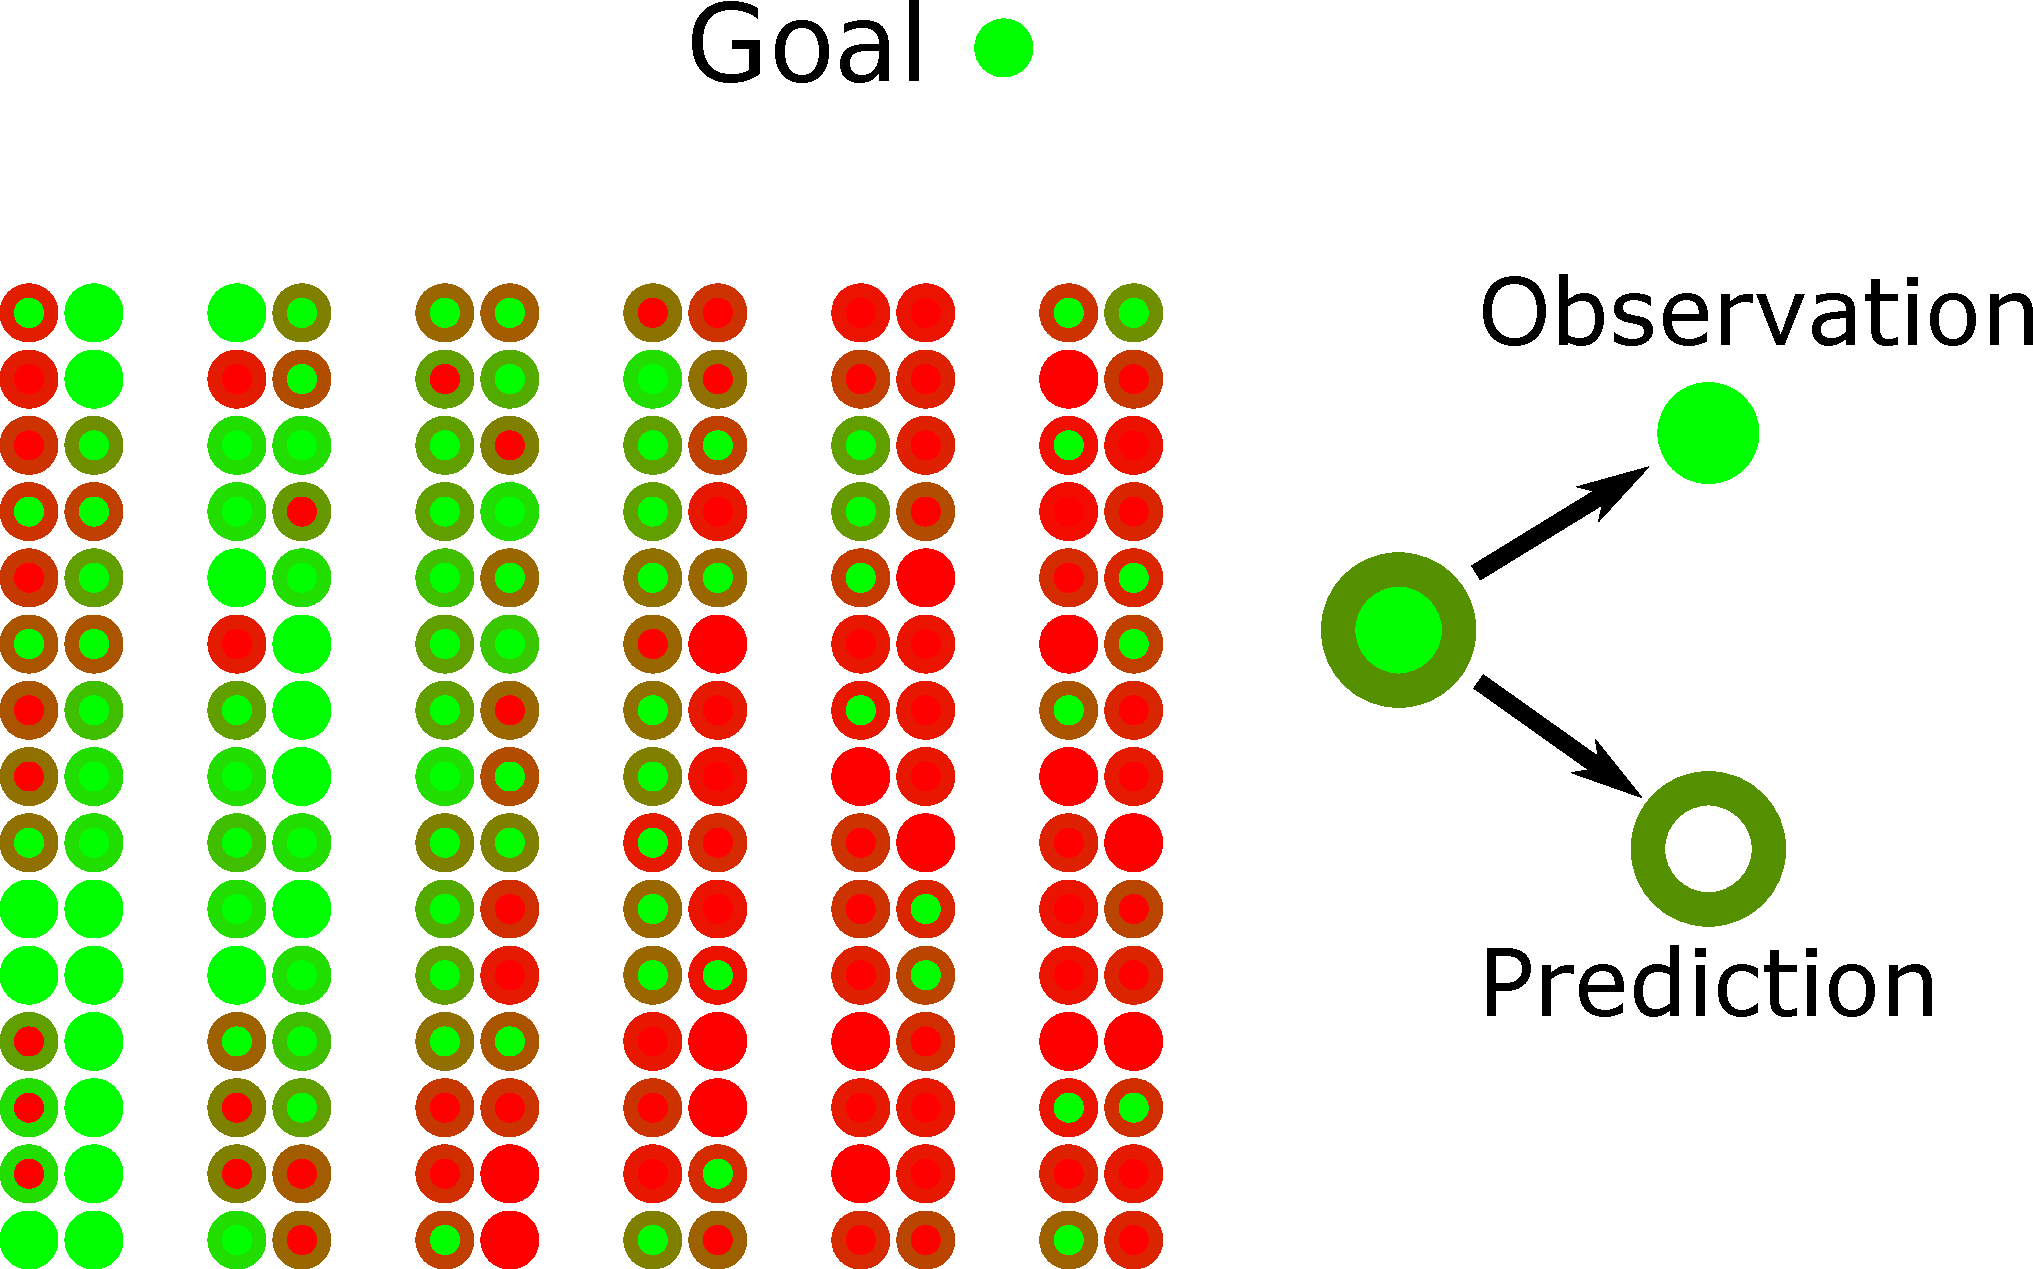
\includegraphics[width=0.5\textwidth]{pictures/graph_observations.pdf}
\end{center}
\caption{A visual representation of the parking lot graph useful for planner visualization. The edges are defined similarly to~\ref{fig:graph}. Each state contains prediction and observation information. This can be seen as combining occupancy information in Figure~\ref{subfig:pre_defined} with Figure~\ref{fig:occupancy_accumulated}.}
\label{fig:graph_accumulated_illustration}
\end{figure}

\begin{figure}[b]%
\centering
\subfloat[Drive up.]{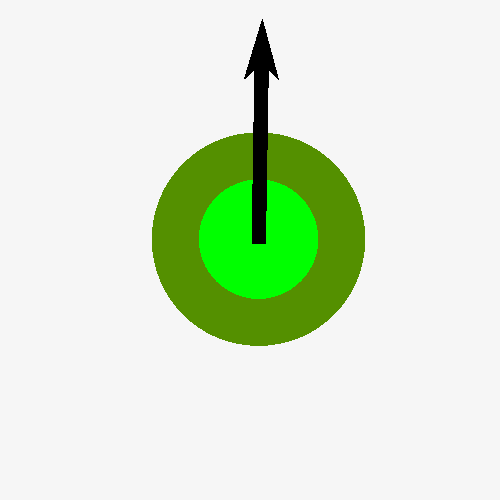
\includegraphics[width=0.15\textwidth]{pictures/action_up.pdf}}\hspace{2mm}
\subfloat[Drive right.]{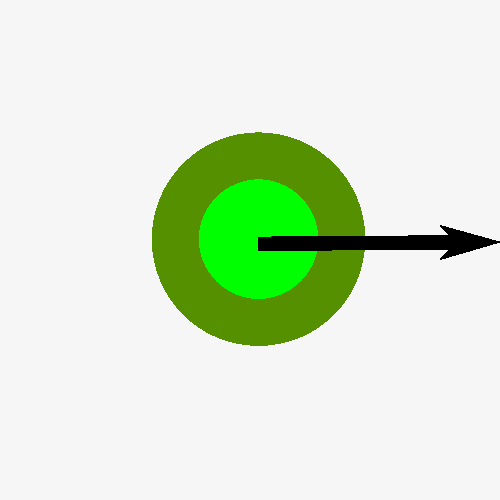
\includegraphics[width=0.15\textwidth]{pictures/action_right.pdf}}\hspace{2mm}
\subfloat[Drive down.]{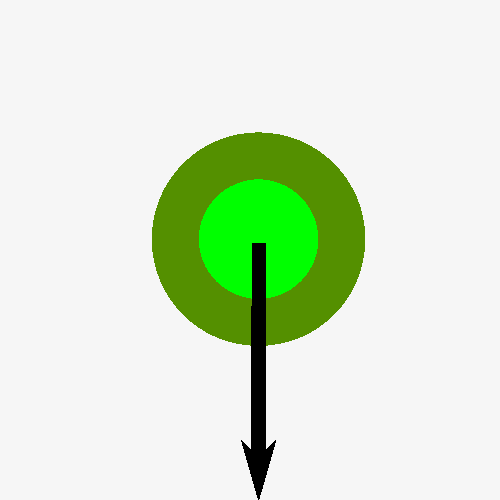
\includegraphics[width=0.15\textwidth]{pictures/action_down.pdf}}\hspace{2mm}
\subfloat[Drive left.]{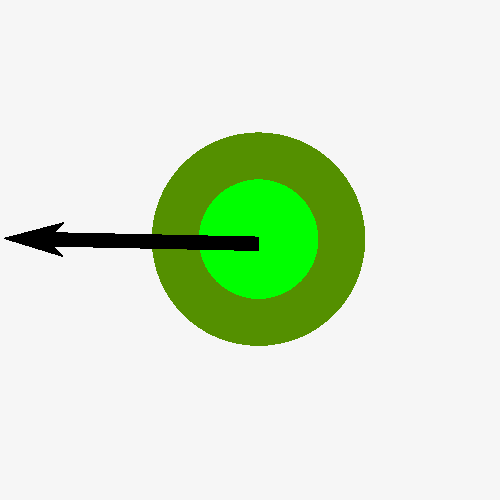
\includegraphics[width=0.15\textwidth]{pictures/action_left.pdf}}\hspace{2mm}
\subfloat[Try to park.]{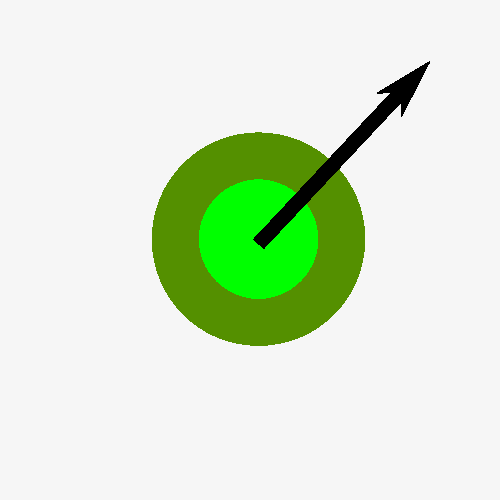
\includegraphics[width=0.15\textwidth]{pictures/action_park.pdf}}
\caption{Visualization of the actions considered optimal by a policy on the graph.}
\label{fig:actions}
\end{figure}

In this section we present the evaluation of the work of the MDP based
planner, that searches for a free parking space. As a testing environment we
use the parking lot at the campus of the University of Freiburg.

We make use of the occupancy information gathered from integrating the
measurements of the parking lots' occupancy (see
Figure~\ref{subfig:pre_defined}) as observed during a period of 21 days. In
order to be able to show the results of the planner we introduce a number of
visualizations. We visualize every parking space as a state in which the agent
can perform an action to park as presented in
Figure~\ref{fig:graph_accumulated_illustration}, where each state shows both
--- the prediction of the occupancy probability as an outer circle and the
actual free or occupied state as the inner one. This representation is useful
to see in a glance what the state of the parking was on the specific date,
while being able to analyze the reasoning behind the agent's actions. However,
only the information shown as an outer circle --- the occupancy prediction is
available to the robot on the planning step. The occupancy prediction is only
then updated to the real occupancy status, when the parking lot is observed by
the agent as he drives by. The actions, that the agent is able to carry out,
as presented in~\eqref{eq:actions} are visualized in the way shown in
Figure~\ref{fig:actions}.

\begin{figure}[tb]
\begin{center}
\subfloat[]{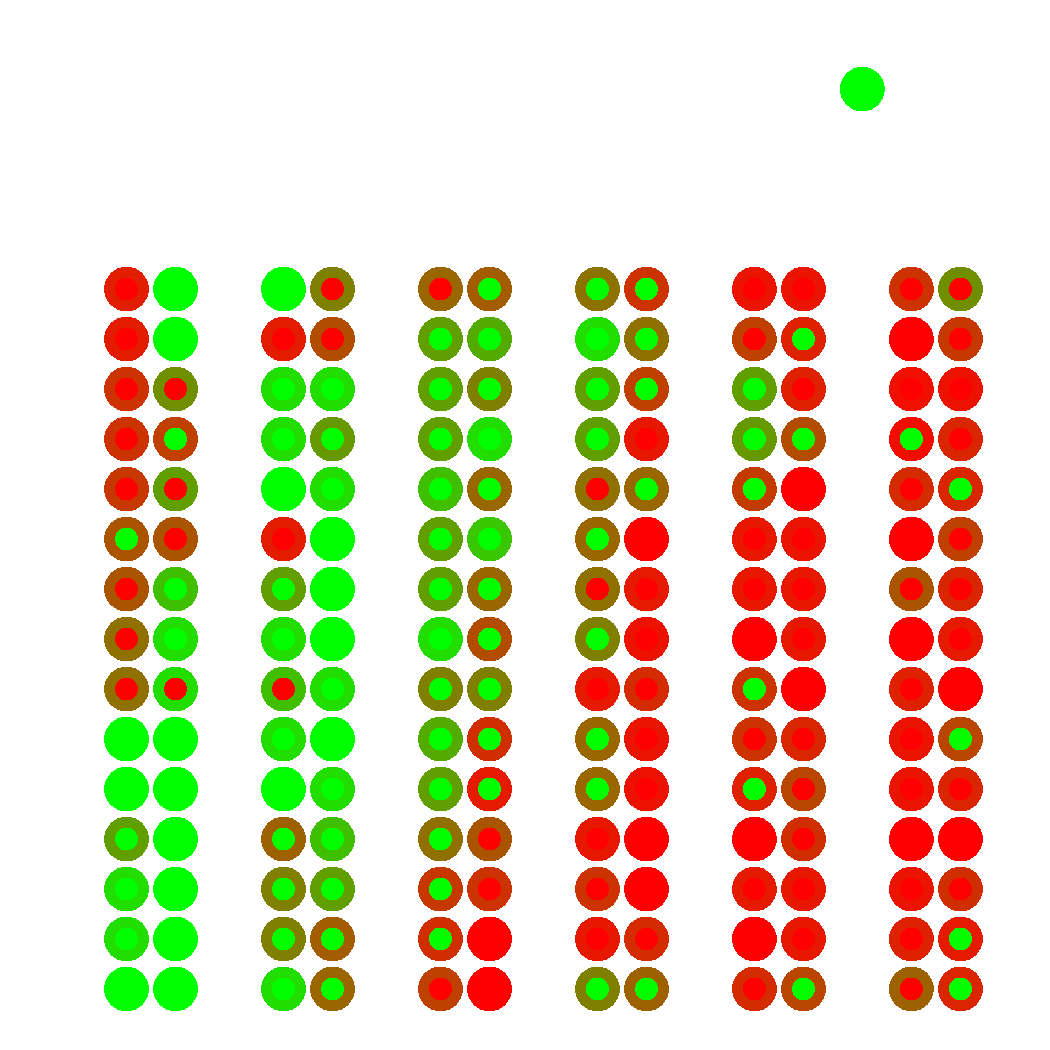
\includegraphics[width=0.45\textwidth]{pictures/walk_4_drive_10_wait_10_data_log_12_12_2013_states.pdf}}\hspace{2mm}
\subfloat[]{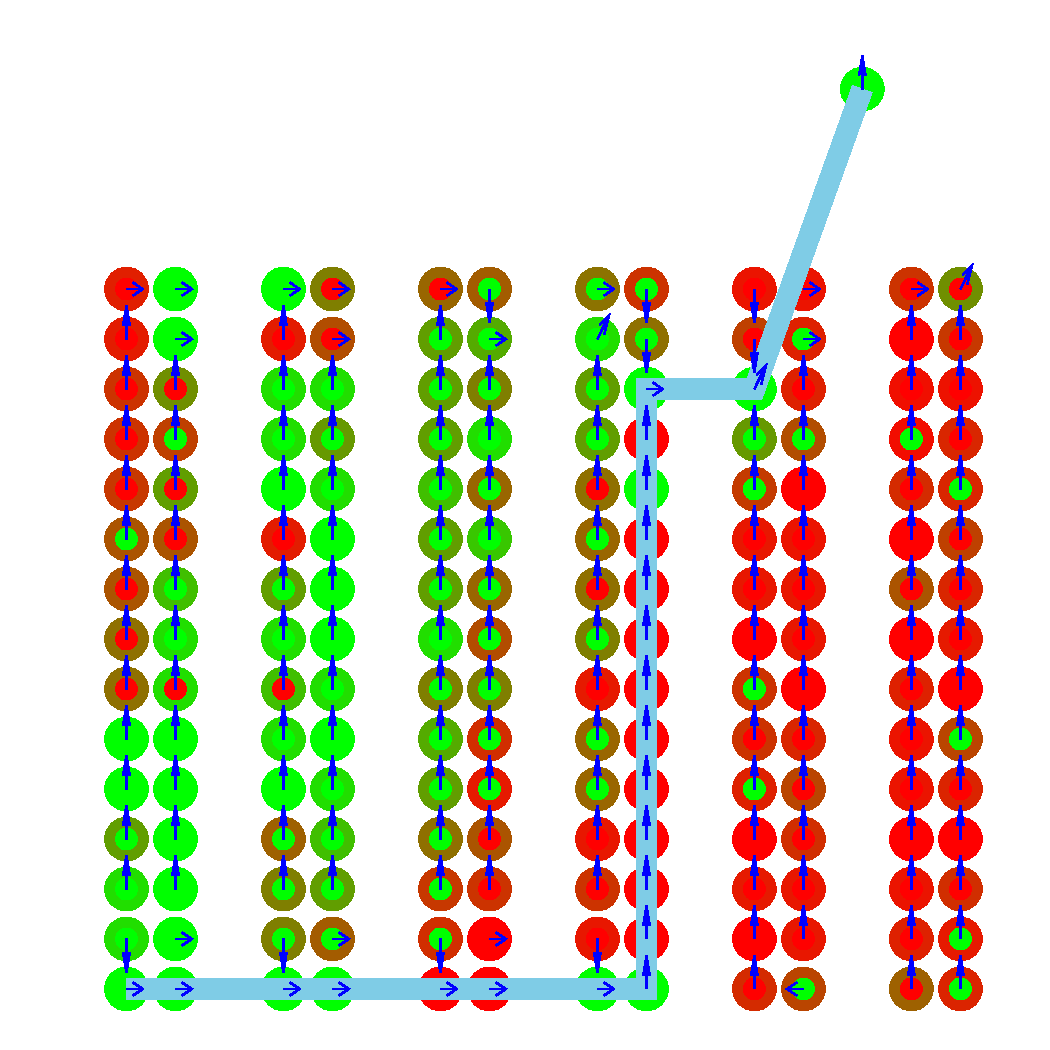
\includegraphics[width=0.45\textwidth]{pictures/walk_4_drive_10_wait_10_data_log_12_12_2013_path_1.pdf}}\hspace{2mm}
\end{center}
\caption{An optimal strategy for $v_{\mathrm{walk}} = 4$ km/h, $v_{\mathrm{drive}} = 10$ km/h and the failure cost of 10 seconds. Each state is presented by an inner and an outer circles. The inner circle depicts the real occupancy status on the day the experiment was held. The outer one presents the occupancy estimate based on the data accumulated from multiple runs. Both circle's colors vary from red for occupied parking lots to green for free ones.}
\label{fig:w_4_d_10_w_10_log_12_12}
\end{figure}

As described in Section~\ref{sec:action_planning} there are 3 core parameters
that influence the performance of the planner: $v_{\mathrm{walk}}$, $v_{\mathrm{drive}}$ and the
failure cost. In this section we present the differences in the behavior of
the agent with respect to different values of these parameters. All the
experiments share the same actual positions of the parked cars for the ease of
comparison.

For these parameters we consider a number of sets of their values. We further
present the differences in the approach picked by the agent depending on the
different sets of the parameters.

\begin{figure}[t]
\begin{center}
\vspace{-5mm}
\subfloat[Initial parking lot state.]{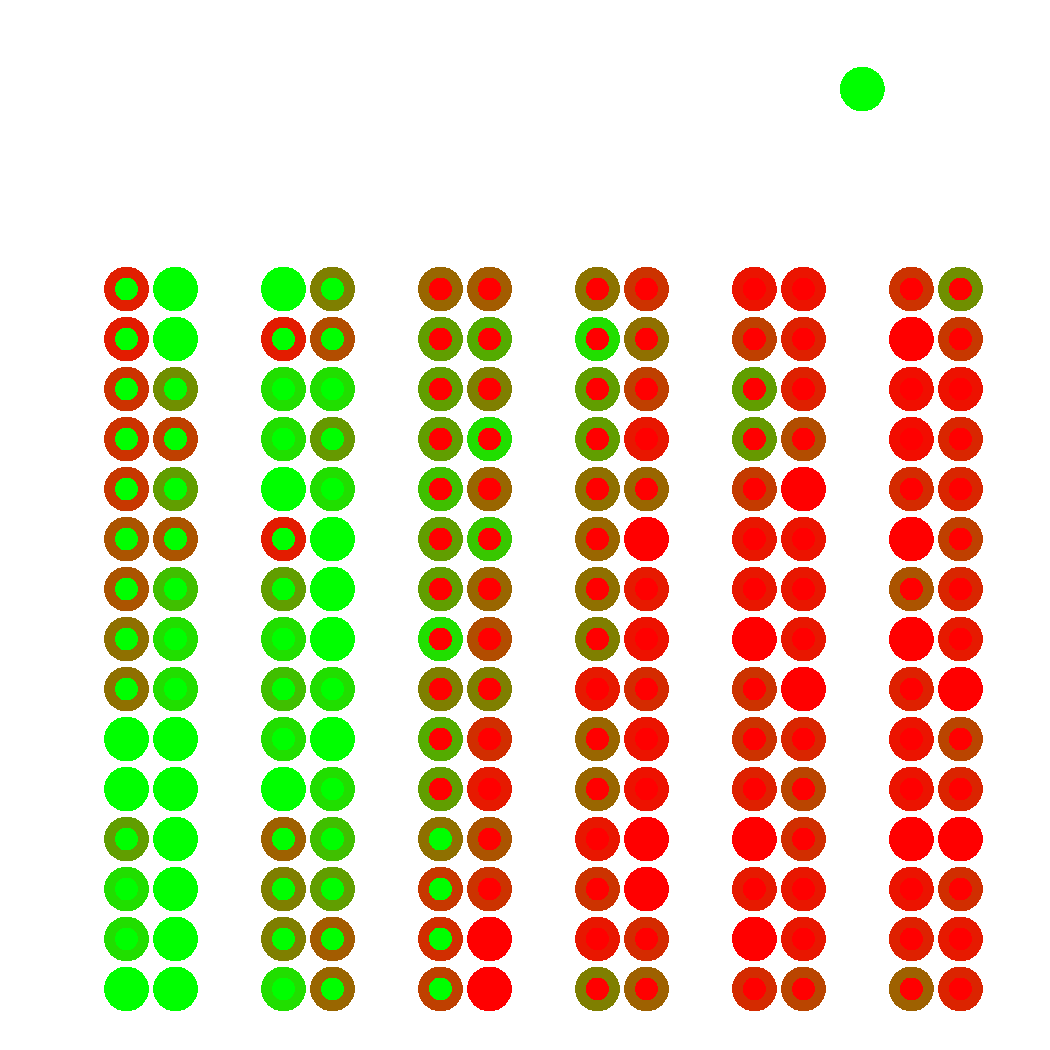
\includegraphics[width=0.35\textwidth]{pictures/walk_4_drive_10_wait_90_data_artificial_states.pdf}}\hspace{2mm}
\subfloat[$1^{st}$ iteration.]{\includegraphics[width=0.35\textwidth]{pictures/walk_4_drive_10_wait_90_data_artificial_path_1.pdf}}\\\vspace{-5mm}
\subfloat[$2^{nd}$ iteration.]{\includegraphics[width=0.35\textwidth]{pictures/walk_4_drive_10_wait_90_data_artificial_path_2.pdf}}\hspace{2mm}
\subfloat[$3^{rd}$ iteration.]{\includegraphics[width=0.35\textwidth]{pictures/walk_4_drive_10_wait_90_data_artificial_path_3.pdf}}\\\vspace{-5mm}
\end{center}
\caption{An optimal strategy for $v_{\mathrm{walk}} = 4$ km/h, $v_{\mathrm{drive}} = 10$ km/h and the failure cost of 90 seconds carried out on an artificial dataset.}
\label{fig:w_4_d_10_w_90_artificial}
\end{figure}

Figure~\ref{fig:w_4_d_10_w_10_log_12_12} shows the path considered optimal by
the agent, given the driving speed of 10 km/h and walking speed of 4 km/h.
Additionally, a failure cost of 10 seconds ensures, that the agent considers
that it loses 10 seconds for every unsuccessful parking action. This results
in the strategy that finds a trade-off between the distance from the parking
lots to the goal and their occupancy. The figure shows that the agent decides
for a state that combines close proximity to the goal state with locally high
probability of being free.

\begin{figure}[t]
\begin{center}
\subfloat[Optimal strategy for $v_{\mathrm{walk}} = 4$ km/h, $v_{\mathrm{drive}} = 10$ km/h and the failure cost of 90 seconds tested on the real data.]{\includegraphics[width=0.40\textwidth]{pictures/walk_2_drive_15_wait_90_data_log_12_12_2013_path_1.pdf}\label{subfig:long_wait_real}}\hspace{6mm}
\subfloat[Optimal strategy for $v_{\mathrm{walk}} = 10$ km/h, $v_{\mathrm{drive}} = 10$ km/h and the failure cost of 90 seconds tested on the real data.]{\includegraphics[width=0.40\textwidth]{pictures/walk_10_drive_10_wait_90_data_log_12_12_2013_path_1.pdf}\label{subfig:fast_walk}}
\end{center}
\caption{}
\label{fig:long_wait_fast_walk}
\end{figure}

Looking at Figure~\ref{fig:w_4_d_10_w_10_artificial} that shows the
performance of the search with the same core parameters on the artificial
dataset we see, that in a rare case of extremely high abnormal occupancy in
the area, the agent is too confident that the parking action would succeed and
it results in extremely long paths and numerous re-planning steps. The agent
tends to pick the places, situated closer to the goal. To deal with this issue
we set the failure cost to a high value, which results in penalizing the
choice of the parking lots in which the agent is likely to fail the parking
action. Setting the failure cost to 90 seconds results in a much more
conservative behavior as presented in
Figure~\ref{fig:w_4_d_10_w_90_artificial}.

Such conservative strategy also proves to be efficient in the real world
scenarios as can be seen in Figure~\ref{subfig:long_wait_real}, showing only a
rare need for re-planning. However, this strategy keeps the agent from making
overly optimistic decisions and he hardly ever observes the most occupied
parts of the parking lot.

Another interesting example that is worth mentioning is the test where human
speed is set to a high value. In the Figure~\ref{subfig:fast_walk} we observe,
that the agent makes the decision that the most practical strategy is to park
in the closest to the starting state parking space and walk to the goal from
there. This is a result of setting $v_{\mathrm{walk}}$ to be equal to $v_{\mathrm{drive}}$. It
may be explained as follows: if the walking speed is equal to the driving
speed it makes no sense driving around the parking lot when it is possible to
walk straight to the goal.


\begin{figure}[tbh]
\begin{center}
\subfloat[Initial parking lot state.]{\includegraphics[width=0.40\textwidth]{pictures/walk_4_drive_10_wait_10_data_artificial_states.pdf}}\hspace{2mm}
\subfloat[$1^{st}$ iteration.]{\includegraphics[width=0.40\textwidth]{pictures/walk_4_drive_10_wait_10_data_artificial_path_1.pdf}}\\
\subfloat[$3^{rd}$ iteration.]{\includegraphics[width=0.40\textwidth]{pictures/walk_4_drive_10_wait_10_data_artificial_path_3.pdf}}\hspace{2mm}
\subfloat[$4^{th}$ iteration.]{\includegraphics[width=0.40\textwidth]{pictures/walk_4_drive_10_wait_10_data_artificial_path_4.pdf}}\\
\subfloat[$16^{th}$ iteration.]{\includegraphics[width=0.40\textwidth]{pictures/walk_4_drive_10_wait_10_data_artificial_path_16.pdf}}\hspace{2mm}
\subfloat[$22^{nd}$ iteration.]{\includegraphics[width=0.40\textwidth]{pictures/walk_4_drive_10_wait_10_data_artificial_path_22.pdf}}
\end{center}
\caption{An optimal strategy for $v_{\mathrm{walk}} = 4$ km/h, $v_{\mathrm{drive}} = 10$ km/h and the failure cost of 10 seconds carried out on an artificial dataset.}
\label{fig:w_4_d_10_w_10_artificial}
\end{figure}
% section planning_results (end)
% chapter experimental_results (end)


%!TEX root = Thesis.tex

\chapter{Conclusion and Further Work} % (fold)
\label{cha:conclusion_and_further_work}

    We have built a system that integrates perception, mapping and planning
    for solving a task of efficient search for a free on-street parking lot.

    The algorithm we present in this work relies on visual detection of the
    cars in the streets. As no reliable fast car detector was found we have
    written one, which is going to be made open-source in the near future.

    Throughout the course of the work we experiment with different methods for
    combining metric information with visual detections such as utilizing
    depth from a stereo camera or a laser range finder. Currently the laser
    range scanner s proven to provide a better result, however it is of great
    interest to build a system that would provide the same level of detail
    adopting purely visual information.

    It is important to have a reliable depth estimate and of the same
    importance is having likewise a good estimate of the position in the
    world. We use SLAM
    (\cite{stachniss11isrr,kuemmerle11auro,kretzschmar10ki}) for estimating a
    precise position of the agent in the world.

    Not only we experiment with perception, but also with mapping. We
    implement the occupancy grids based approach, which, however, suffers from
    the discretization errors as well as from ad-hoc estimation of the
    position (including orientation) of the detected cars in the occupancy
    grid. Eventually we promote the system where we provide our system with
    additional knowledge about where the parking lots are situated. This
    information has to be obtained only once for a new environment.

    This system then provides a good estimate of the occupancy information
    that we estimate via multiple observations of the same spot on different
    days or simply in different times. It may be a subject for future work to
    estimate the occupancy information for particular day of week or
    particular time of a working day, etc. The occupancy information is
    basically a probability of a parking lot to be free when observed.

    This occupancy information along with the position of the parking lots in
    the world allows us to introduce a planner. This planner, unlike greedy A*
    and alike, searches not for the best parking lot in the means of position
    or occupancy, but takes into account the trade-off between these two
    quantities, minimizing the expected time required by an agent to park a
    car and get to the final goal by foot. It is still possible to experience
    difficulties finding the best parking lot, but our approach eliminates the
    high uncertainty of this process and provides an opportunity to carry out
    the parking process in a fully-autonomous fashion, while guaranteeing to
    find the best action in the means of expected time needed for the whole
    process.

    There is however place for future work. To see a fully integrated and
    easily accessible system we will further focus on detecting the parked car
    position purely based on visual data (via improving stereo-camera depth
    acquisition). The other vector of interest is improving the approach for
    mapping in order to leave pre-defined parking lots' positions behind and
    to be able to efficiently map any given environment without any prior
    knowledge about it.

% chapter conclusion_and_further_work (end)


%\bibliographystyle{ieeetr}
\cleardoublepage
\phantomsection \label{chap:bibliography}
\addcontentsline{toc}{chapter}{Bibliography}
\bibliographystyle{plainnat}

\bibliography{refs}
\end{document}

